\documentclass[12pt]{iopart}
%\usepackage{ucs}
%\usepackage{amsmath,amssymb,amsthm}
\usepackage{iopams,amssymb,amsthm}
%\usepackage{pb-diagram}
\usepackage{multicol}
%\usepackage[utf8x]{inputenc}
%\usepackage[russian]{babel}
\usepackage{cmap}
\usepackage{color}
%\usepackage[pdftex]{graphicx}
\usepackage{graphicx}
%\pagestyle{plain}
%\usepackage[unicode,verbose,plainpages=false]{hyperref}
\usepackage{hyperref}

%\usepackage{verbatim}
%\newenvironment{comment}
%{\par\noindent{\bf TODO}\\}
%{\\\hfill$\scriptstyle\blacksquare$\par}

\newtheorem{statement}{Statement}
\newtheorem{lemma}{Lemma}
\newtheorem{theorem}{Theorem}
\theoremstyle{definition}
\newtheorem{corollary}{Corollary}[theorem]
\theoremstyle{definition}
\newtheorem{mynote}{Note}[section]
\theoremstyle{definition}
\newtheorem{definition}{Definition}
\newcommand{\go}{\stackrel{\circ }{\mathfrak{g}}}
\newcommand{\ao}{\stackrel{\circ }{\mathfrak{a}}}
\newcommand{\co}[1]{\stackrel{\circ }{#1}}

\begin{document}

\title{Recursive algorithms, branching coefficients and applications}
\author{V D Lyakhovsky$^1$ and A A Nazarov$^2$}
\address{$^{1,2}$ Theoretical Department, SPb State University,
198904, Sankt-Petersburg, Russia }
\eads{$^1$ \mailto{lyakh1507@nm.ru}, $^2$ \mailto{antonnaz@gmail.com}}

\begin{abstract}
  Recurrent relations for branching coefficients in affine Lie algebras integrable highest weight modules are studied. The decomposition algorithm based on the injection fan technique is adopted to the situation where the Weyl denominator becomes singular with respect to a reductive subalgebra. We study some modifications of the injection fan technique and demonstrate that it is possible to define the "subtracted fans" that play the role similar to the original ones. Possible applications of subtracted fans in CFT models are considered.
\end{abstract}
\ams{17B67, 17B10}
\submitto{\JPA}
%\maketitle

\section{Introduction}
\label{sec:introduction}

The branching problem for affine Lie algebras emerges in conformal field theory, for example,
in the construction of modular-invariant partition functions \cite{difrancesco1997cft}.
Recently the problem of conformal embeddings was considered in the paper \cite{coquereaux2008conformal}.

There exist several approaches to deal with the branching coefficients. Some of them use the BGG
resolution \cite{bernstein1975differential} (for Kac-Moody algebras the algorithm is described in
\cite{kac1990idl},\cite{wakimoto2001idl}), the Schure function series \cite{fauser2006new}, the BRST
cohomology \cite{Hwang:1994yr}, Kac-Peterson formulas \cite{kac1990idl,quella2002branching} or the
combinatorial methods applied in \cite{feigin707principal}.

Usually only the maximal reductive subalgebras are considered since the case of non-maximal subalgebra
can be obtained using the chain of maximal injections. In this paper we find the recurrent properties
for branching coefficients that generalize the relations obtained earlier (see the paper \cite{ilyin812pbc}
and the references therein) to the case of non-maximal reductive subalgebra. The result is formulated in
terms of the new injection fan called "the subtracted fan". Using this new tools we formulate a simple and
explicit algorithm for computations of branching coefficients which is applicable to the non-maximal
subalgebras of finite-dimensional and affine Lie algebras.

We demonstrate that our algorithm can be used in studies of conformal embeddings and coset constructions
in rational conformal field theory.

The paper is organised as follows. In the subsection \ref{sec:notation}  we fix the notations.
In the Section \ref{sec:recurr-form-branch} we derive the subtracted recurrent formula for anomalous
branching coefficients and describe the decomposition algorithm for integrable highest weight modules
$L_{\mathfrak{g}}$ with respect to a reductive subalgebra $\mathfrak{a}\subset \mathfrak{g}$
(subsection \ref{sec:algorithm}). In the Section \ref{sec:finite-dimens-lie} we present several
simple examples for finite-dimensional Lie algebras. The affine Lie algebras and their applications in
CFT models are considered in Section \ref{sec:phys-appl}.
Possible further developments are discussed (Section \ref{sec:conclusion}).

\subsection{Notation}
\label{sec:notation}

Consider affine Lie algebras $\frak{g}$ and $\frak{a}$ with the
underlying finite-dimensional subalgebras $\go$ and $%
\ao$ and an injection $\frak{a}\longrightarrow \frak{g%
}$ such that $\frak{a}$ is a reductive subalgebra $\frak{a\subset g}$ with
correlated root spaces: $\frak{h}_{\frak{a}}^{\ast }\subset \frak{h}_{\frak{g%
}}^{\ast }$ and $\frak{h}_{\ao}^{\ast }\subset \frak{h%
}_{\go}^{\ast }$\ .

We use the following notations:

$L^{\mu }$\ $\left( L_{\frak{a}}^{\nu }\right) $\ --- the integrable module
of $\frak{g}$ with the highest weight $\mu $\ ; (resp. integrable $\frak{a}$
-module with the highest weight $\nu $ );

$r$ , $\left( r_{\frak{a}}\right) $ --- the rank of the algebra $\frak{g}$ $%
\left( \mbox{resp. }\frak{a}\right) $ ;

$\Delta $ $\left( \Delta _{\frak{a}}\right) $--- the root system; $\Delta
^{+} $ $\left( \mbox{resp. }\Delta _{\frak{a}}^{+}\right) $--- the positive
root system (of $\frak{g}$ and $\frak{a}$ respectively);

$\mathrm{mult}\left( \alpha \right) $ $\left( \mathrm{mult}_{\frak{a}}\left(
\alpha \right) \right) $ --- the multiplicity of the root $\alpha$ in $\Delta
$ (resp. in $\left( \Delta _{\frak{a}}\right) $);

$\co{\Delta}$ , $\left( \co{\Delta _{\frak{a}}}%
\right)$ --- the finite root system of the subalgebra $\co{%
\frak{g}}$ (resp. $\co{\frak{a}}$);
$\Theta$, $(\Theta_{\mathfrak{a}})$ --- the highest root of the algebra $\mathfrak{g}$ (resp. subalgebra $\mathfrak{a}$);

$\mathcal{N}^{\mu }$ , $\left( \mathcal{N}_{\frak{a}}^{\nu }\right) $ --- the
weight diagram of $L^{\mu }$ $\left( \mbox{resp. }L_{\frak{a}}^{\nu }\right)
$ ;

$W$ , $\left( W_{\frak{a}}\right) $--- the corresponding Weyl group;

$C$ , $\left( C_{\frak{a}}\right) $--- the fundamental Weyl chamber;

$\bar{C}, \left(\bar{C_{\mathfrak{a}}}\right)$ --- the closure of the fundamental Weyl chamber;

$\rho $\ , $\left( \rho _{\frak{a}}\right) $\ --- the Weyl vector;

$\epsilon \left( w\right) :=\det \left( w\right) $ ;

$\alpha _{i}$ , $\left( \alpha _{\left( \frak{a}\right) j}\right) $ --- the $i
$-th (resp. $j$-th) basic root for $\frak{g}$ $\left( \mbox{resp. }\frak{a}%
\right) $; $i=0,\ldots ,r$,\ \ $\left( j=0,\ldots ,r_{\frak{a}}\right) $;

$\delta $ --- the imaginary root of $\frak{g}$ (and of $\frak{a}$ if any);

$\alpha _{i}^{\vee }$ , $\left( \alpha _{\left( \frak{a}\right) j}^{\vee
}\right) $--- the basic coroot for $\frak{g}$ $\left( \mbox{resp. }\frak{a}%
\right) $ , $i=0,\ldots ,r$ ;\ \ $\left( j=0,\ldots ,r_{\frak{a}}\right) $;

$\co{\xi }$ , $\co{\xi _{\left( \frak{a}\right) }}$
--- the finite (classical) part of the weight $\xi \in P$ , $\left( \mbox{%
resp. }\xi _{\left( \frak{a}\right) }\in P_{\frak{a}}\right) $;

$\lambda =\left( \co{\lambda };k;n\right) $ --- the
decomposition of an affine weight indicating the finite part $\co{\lambda }$, level $k$ and grade $n$;

$P$ $\left( \mbox{resp. } P_{\frak{a}}\right) $ \ --- the weight lattice;

$M \left( \mbox{resp. }M_{\frak{a}}\right) :=$

\noindent $=\left\{
\begin{array}{c}
\sum_{i=1}^{r}\mathbf{Z}\alpha _{i}^{\vee }\mbox{ }\left( \mbox{resp. }%
\sum_{i=1}^{r}\mathbf{Z}\alpha _{\left( \frak{a}\right) i}^{\vee }\right)
\mbox{for untwisted algebras or }A_{2r}^{\left( 2\right) }, \\
\sum_{i=1}^{r}\mathbf{Z}\alpha _{i}\mbox{ }\left( \mbox{resp. }\sum_{i=1}^{r}%
\mathbf{Z}\alpha _{\left( \frak{a}\right) i}\right) \mbox{for }A_{r}^{\left(
u\geq 2\right) }\mbox{ and }A\neq A_{2r}^{\left( 2\right) },
\end{array}
\right\} ;$\\
$\Psi ^{\left( \mu \right) }:=\sum\limits_{w\in W}\epsilon (w)e^{w\circ (\mu +\rho )-\rho }$ --- the singular weight element for the $\frak{g}$-module $L^{\mu }$;
$\Psi _{\left( \frak{a}\right) }^{\left( \nu \right) }:=\sum\limits_{w\in W_{\frak{a}}}\epsilon (w)e^{w\circ (\nu +\rho
_{_{\frak{a}}})-\rho _{_{\frak{a}}}}$ --- the corresponding singular weight
element for the $\frak{a}$-module $L_{\frak{a}}^{\nu }$;

$\widehat{\Psi ^{\left( \mu \right) }}$ $\left( \widehat{\Psi _{\left( \frak{%
a}\right) }^{\left( \nu \right) }}\right) $ --- the set of singular weights $%
\xi \in P$ $\left( \mbox{resp. }\in P_{\frak{a}}\right) $ for the module $%
L^{\mu }$ $\left( \mbox{resp. }L_{\frak{a}}^{\nu }\right) $ with the
coordinates $\left( \co{\xi },k,n,\epsilon \left( w\left( \xi
\right) \right) \right) \mid _{\xi =w\left( \xi \right) \circ (\mu +\rho
)-\rho },$ (resp. $\left( \co{\xi },k,n,\epsilon \left(
w_{a}\left( \xi \right) \right) \right) \mid _{\xi =w_{a}\left( \xi \right)
\circ (\nu +\rho _{a})-\rho _{a}}$ );

$m_{\xi }^{\left( \mu \right) }$ , $\left( m_{\xi }^{\left( \nu \right)
}\right) $ --- the multiplicity of the weight $\xi \in P$ \ $\left( \mbox{%
resp. }\in P_{\frak{a}}\right) $ in the module $L^{\mu }$ , (resp. $\xi \in
L_{\frak{a}}^{\nu } $);

$ch\left( L^{\mu }\right) $ $\left( \mbox{resp. }ch\left( L_{\frak{a}}^{\nu
}\right) \right) $--- the formal character of $L^{\mu }$ $\left( \mbox{resp. }%
L_{\frak{a}}^{\nu }\right) $;

$ch\left( L^{\mu }\right) =\frac{\sum_{w\in W}\epsilon (w)e^{w\circ (\mu
+\rho )-\rho }}{\prod_{\alpha \in \Delta ^{+}}\left( 1-e^{-\alpha }\right) ^{%
\mathrm{{mult}\left( \alpha \right) }}}=\frac{\Psi ^{\left( \mu \right) }}{%
\Psi ^{\left( 0\right) }}$ --- the Weyl-Kac formula;

$R:=\prod_{\alpha \in \Delta ^{+}}\left( 1-e^{-\alpha }\right) ^{\mathrm{{%
mult}\left( \alpha \right) }}=\Psi ^{\left( 0\right) }\quad $;

\noindent $\left( \mbox{resp. }R_{\frak{a}}:=\prod_{\alpha \in \Delta _{%
\frak{a}}^{+}}\left( 1-e^{-\alpha }\right) ^{\mathrm{mult}_{\frak{a}}\mathrm{%
\left( \alpha \right) }}=\Psi _{\frak{a}}^{\left( 0\right) }\right) $--- the
denominator;

$  L_{\frak{g}\downarrow \frak{a}}^{\mu }=\bigoplus
\limits_{\nu \in P_{\frak{a}}^{+}}b_{\nu }^{\left( \mu \right) }L_{\frak{a}}^{\nu }$
 --- the module decomposition with respect to $\frak{a}\longrightarrow \frak{g}$;


$b^{(\mu)}_{\nu}$ --- the branching coefficients,

\begin{equation}
  \label{eq:21}
  \sum_{\nu \in \bar{C_{\mathfrak{a}}}}b_{\nu }^{\left( \mu \right) }\Psi _{\left( \frak{%
        a}\right) }^{\left( \nu \right) }=\sum_{\lambda \in P_{\frak{a}}}k_{\lambda
  }^{\left( \mu \right) }e^{\lambda };
\end{equation}

 $k_{\lambda}$ --- the anomalous branching coefficients, notice that
\begin{equation*}
%  \label{eq:20}
  b^{(\mu)}_{\nu}=k^{(\mu)}_{\nu} \; \mbox{for} \; \nu\in \bar{C}_{\mathfrak{a}};
\end{equation*}

$x_e=\frac{\left|\pi_{\mathfrak{a}} \Theta\right|^2}{\left|\Theta_{\mathfrak{a}}\right|^2}$ --- the embedding index.

\section{Recurrent relation for branching coefficients. Singularities and subtractions}
\label{sec:recurr-form-branch}

We consider an injection of affine Lie algebras $\frak{a}\longrightarrow \frak{g%
}$ such that $\frak{a}$ is a reductive subalgebra $\frak{a\subset g}$.
In this section we deduce the general recurrent relation (\ref{eq:1}) for the anomalous branching coefficients (\ref{eq:21}). This relation is then used to formulate the practical computational algorithm (Subsection \ref{sec:algorithm}).
In the earlier paper \cite{ilyin812pbc} the following limited setup was considered: $\mathfrak{a}$ was required to be the maximal subalgebra of $\mathfrak{g}$ so that no zeros arrive in the Weyl denominator $R$. Here we raise this limitation and study the general case $\mathfrak{a}\subset\mathfrak{g}$. 

\subsection{Some definitions}
\label{sec:some-definitions}

We need to introduce several additional definitions and state some technical results to formulate and prove the recurrent relation (\ref{eq:1}).

\begin{definition}
  Denote by $\Delta^{+}_{\bot}=\left\{\alpha\in \Delta^{+}_{\mathfrak{g}}:\forall \beta\in\Delta_{\mathfrak{a}} \; \alpha\bot \beta\right\}$ the subset of the positive roots of $\mathfrak{g}$ orthogonal to the root system of $\mathfrak{a}$.
\end{definition}

\begin{definition}
  Denote by $W_{\bot}$ the subgroup of the Weyl group $W$ generated by the reflections $\omega_{\alpha}$ corresponding to the roots $\alpha\in \Delta^{+}_{\bot}$.
\end{definition}
\begin{mynote}
  The subgroup $W_{\bot}$ preserves $\Delta_{\mathfrak{a}}$ since it is generated by the reflections in hyperplanes containing $\Delta_{\mathfrak{a}}$.
\end{mynote}
\begin{definition}
  The subsystem $\Delta_{\bot}=\Delta^{+}_{\bot}\cup \left(-\delta^{+}_{\bot}\right)$ determines the subalgebra $\mathfrak{a}_{\bot}\subset \mathfrak{g}$.
\end{definition}

We need to know when the subset $\Delta^{+}_{\bot}$ is non-empty and $W_{\bot},\mathfrak{a}_{\bot}$ are non-trivial. So we state several simple lemmas.

For the simple finite-dimensional Lie algebras $\ao,\go$ all the regular embeddings can be obtained by the successive elimination of the nodes in the extended Dynkin diagram of $\go$. This leads to the lemma
\begin{lemma}
  For the regular embedding $\ao\subset \go$ 
  \renewcommand{\theenumi}{\alph{enumi}}
  \begin{enumerate}
  \item $\Delta^{+}_{\bot}=\emptyset$ if $\ao$ is maximal
  \item If the extended Dynkin diagram of $\go$ contains the disconnected subdiagrams of $\ao$ and some subalgebras $\left\{\co{\mathfrak{a}_j}\right\}$ then $\Delta^{+}_{\bot}\neq \emptyset$ and $\co{\mathfrak{a}_j}\subset \mathfrak{a}_{\bot}$.
  \end{enumerate}
\end{lemma}
\begin{mynote}
  The complete classification of the regular subalgebras for affine Lie algebras can be
  found in the recent paper \cite{1751-8121-41-36-365204}.
\end{mynote}
\begin{mynote}
  $\mathfrak{a}_{\bot}$ may be larger than the algebra $\bigoplus_j \co{\mathfrak{a}_j}$.
\end{mynote}
Consider for example the embedding of $B_2\subset B_4$ (the Figure \ref{fig:dynkin}).
In this case by eliminating
the simple root $\alpha_2=e_2-e_3$ one splits the extended Dynkin diagram of $B_4$
into the diagrams of the subalgebra $\mathfrak{a}=B_2$ and that of the direct
sum $A_1 \oplus A_1 $. But the subalgebra $\mathfrak{a}_{\bot}$ is equal to $B_2$
(the root system of $B_4$ contains not only $\alpha_2=e_2-e_3$ but also $e_2$).

Such effects are due to the fact that the subalgebras $\mathfrak{a}$ and $\mathfrak{a}_{\bot}$
must not form a direct sum in $\mathfrak{g}$.
Consider the case of such a regular embedding $\mathfrak{a}\subset \mathfrak{g}$ where both
algebras are simple and the diagram of the subalgebra $\mathfrak{a}_{\bot}$ is not a
subdiagram of the extended Dynkin diagram $\mathfrak{g}$.
Drop the subdiagram of $\mathfrak{a}$ and the node $\alpha'$ that connects it with
the remaining nodes of the diagram of $\mathfrak{g}$. The result is the diagram of
the algebra $\bar{\mathfrak{a}}$ with $\mathrm{rank}(\bar{\mathfrak{a}}) =
\mathrm{rank}(\mathfrak{g})-\mathrm{rank}(\mathfrak{a})$. It is clear that
$\bar{\mathfrak{a}}\subset \mathfrak{a}_{\bot}$. So the question is whether
$\mathfrak{a}_{\bot}$ has additional roots,  not the roots of $\bar{\mathfrak{a}}$
but the linear combinations of them. The answer is positive  when the set of angles
between the roots of $\bar{\mathfrak{a}}$ does not contain all the angles between
the roots of $\mathfrak{a}$.
Then by reflecting the roots of $\mathfrak{a}$ by $s_{\alpha'}$ we get the additional
roots of $\mathfrak{a}_{\bot}$.
Case-by-case analysis illustrated by the table \ref{tab:diagrams} leads us to the following lemma.

\begin{table}[h!tb]
\label{tab:diagrams}
\noindent  \centering{
\begin{tabular}{|l|l|l|l|}
  \hline
  $\mathfrak{g}$ & Extended diagram of $\mathfrak{g}$ &
  Diagrams of the subalgebras $\mathfrak{a},\; \mathfrak{a}_{\bot}$ \\
  \hline
  $A_n$ & 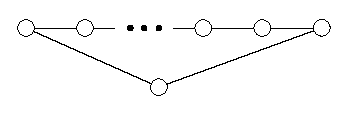
\includegraphics{table1_1(l).eps} & 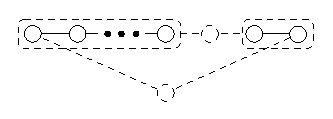
\includegraphics{table1_1(r).eps} \\
  \hline
  $B_n$ & 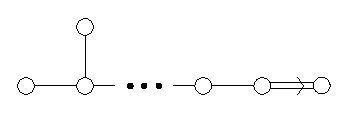
\includegraphics{table1_2(l).eps} & 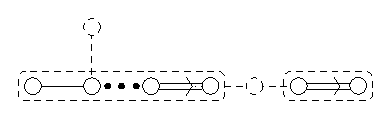
\includegraphics{table1_2(r).eps} \\
  \hline
  $C_n$ & 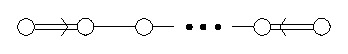
\includegraphics{table1_3(l).eps} & 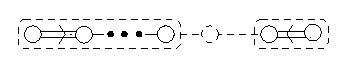
\includegraphics{table1_3(r).eps} \\
  \hline
  $D_n$ & 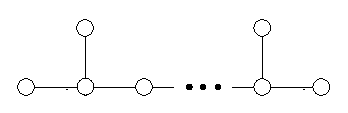
\includegraphics{table1_4(l).eps} & 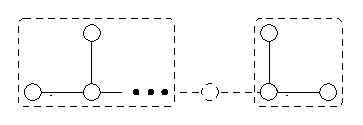
\includegraphics{table1_4(r).eps} \\
  \hline
\end{tabular}
\caption{Subalgebras $\mathfrak{a},\; \mathfrak{a}_{\bot}$ for the classical series}}
\end{table}

\begin{lemma}
  \renewcommand{\theenumi}{\alph{enumi}}
  \begin{enumerate}
  \item If $\go,\ao\neq B_r$ the Dynkin diagram of $\mathfrak{a}_{\bot}$ is obtained from the extended Dynkin diagram of $\go$ by dropping the subdiagram of $\ao$ and the adjacent nodes
  \item If $\go=B_r$ and $\ao=B_{r_{\mathfrak{a}}}$ then $\mathfrak{a}_{\bot}=B_{r-r_{\mathfrak{a}}}$.
  \end{enumerate}
\end{lemma}
The complete classification of maximal special subalgebras in classical Lie algebras
\cite{dynkin1952semisimple} allows us to formulate
\begin{lemma}
  For the special embeddings there exist the following set of pairs of orthogonal subalgebras $\mathfrak{a},\;\mathfrak{a}_{\bot}$:
\begin{equation*}
%  \label{eq:42}
  \begin{array}{lll}
      su(p)\oplus su(q) & \subset su(pq) &\\
      so(p)\oplus so(q) & \subset so(pq) &\\
      sp(2p)\oplus sp(2q) & \subset so(4pq)&\\
      sp(2p)\oplus so(q) & \subset sp(2pq)&\\
      so(p)\oplus so(q) & \subset so(p+q)& \mbox{for}\;p\;\mbox{and}\;q\;\mbox{odd}.\\
  \end{array}
\end{equation*}
\end{lemma}
We are almost ready to state and prove the recurrent relation for the anomalous branching coefficients.
\begin{definition}
  \label{fan-definition}
  For affine $\mathfrak{a}\subset\mathfrak{g}$ expand the product
  \begin{equation*}
    \label{eq:6}
    \prod_{\alpha\in \Delta^{+}\setminus\Delta^{+}_{\bot}}
    \left(1-e^{-\pi_{\mathfrak{a}}\alpha}\right)^{
        \mathrm{mult}(\alpha)-\mathrm{mult}_{\mathfrak{a}}(\pi_{\mathfrak{a}}\alpha)}=
      -\sum_{\gamma\in P_{\mathfrak{a}}}e^{-\gamma}
  \end{equation*}
  Denote by $\Phi_{\mathfrak{a}\subset\mathfrak{g}}\subset P_{\mathfrak{a}}$ the carrier of the coefficient function $s(\gamma)$. 
  \begin{equation*}
    \label{eq:37}
    \Phi_{\mathfrak{a}\subset\mathfrak{g}}=\left\{\gamma\in P_{\mathfrak{a}}|s(\gamma)\neq 0\right\}
  \end{equation*}

  The ordering of roots in $\co{\Delta_{\mathfrak{a}}}$ induce the natural ordering on the weights of $\mathfrak{a}$. Denote by $\gamma_0$ the lowest vector of $    \Phi_{\mathfrak{a}\subset\mathfrak{g}}$ according to this ordering. 
  The set 
  \begin{equation}
    \Gamma _{\frak{a}\subset \frak{g}}=\left\{ \xi -\gamma _{0}|\xi \in \Phi _{%
        \frak{a}\subset \frak{g}}\right\} \setminus \left\{ 0\right\}
    \label{fan-defined}
  \end{equation}
  is called the {\it injection fan}.
\end{definition}

\subsection{Proof of the recurrent relation}
\label{sec:proof}
\begin{theorem}
  For the anomalous branching coefficients (\ref{eq:21}) holds the recurrent relation
  \begin{equation}
    \label{eq:1}
    \begin{array}{c}
      k_{\xi }^{\left( \mu \right) }=-\frac{1}{s\left( \gamma _{0}\right) }\left(
        \sum_{\omega\in W_{\bot}\backslash W} \epsilon(\omega)\;
        {\rm dim}\left(L^{\pi_{\mathfrak{a}_{\bot}}(\omega(\mu+\rho))-\rho_{\mathfrak{a}_{\bot}}}_{\mathfrak{a}_{\bot}}\right)
        \delta_{\xi-\gamma_0,\pi_{\mathfrak{a}}(\omega(\mu+\rho)-\rho)}+ \right.\\
      \left.
        +\sum_{\gamma \in
          \Gamma _{\frak{a}\subset \frak{g}}}s\left( \gamma +\gamma _{0}\right) k_{\xi
          +\gamma }^{\left( \mu \right) }\right).
    \end{array}
  \end{equation}
  \begin{proof}
    Consider the branching of a module $L_{\frak{g}}^{\mu }$ in terms of formal characters and
    projection operators $\pi_{\mathfrak{a}}:P\to P_{\mathfrak{a}}$:
    \begin{equation*}
      % \label{eq:3}
      L_{\frak{g}\downarrow \frak{a}}^{\mu }=\bigoplus\limits_{\nu \in P_{\frak{a}%
        }^{+}}b_{\nu }^{\left( \mu \right) }L_{\frak{a}}^{\nu }\quad
      \Longrightarrow\quad
      \pi_{\mathfrak{a}}(ch L^{\mu}_{\mathfrak{g}})=
      \sum_{\nu\in P^{+}_{\mathfrak{a}}}b^{(\mu)}_{\nu} ch L^{\nu}_{\mathfrak{a}}.
    \end{equation*}
    The Weyl-Kac character formula leads to
    the relation
    \begin{equation}
      \label{eq:4}
      \pi_{\mathfrak{a}}\left(\frac{\sum_{\omega\in W} \epsilon(\omega) e^{\omega(\mu+\rho)-\rho}}
        {\prod_{\alpha\in\Delta^{+}}(1-e^{-\alpha})^{\mathrm{mult}(\alpha)}}\right) =
      \sum_{\nu\in P^{+}_{\mathfrak{a}}}b^{(\mu)}_{\nu}
      \frac{\sum_{\omega\in W_{\mathfrak{a}}}\epsilon(\omega)
        e^{\omega(\nu+\rho_{\mathfrak{a}})-\rho_{\mathfrak{a}}}}
      {\prod_{\beta\in \Delta_{\mathfrak{a}}^{+}}(1-e^{-\beta})^{\mathrm{mult}_{\mathfrak{a}}(\beta)}}.
    \end{equation}

    Consider the direct sum $\mathfrak{a}_{\bot}\oplus\mathfrak{h}_{\mathfrak{a}}$ and
    its module $L^{\mu}_{\mathfrak{a}_{\bot}\oplus \mathfrak{h}}$
    with the highest weight $\mu$. The character $ch L^{\mu}_{\mathfrak{a}_{\bot}\oplus \mathfrak{h}}$
    can be written as
    \begin{equation*}
      % \label{eq:41}
      ch L^{\mu}_{\mathfrak{a}_{\bot}\oplus \mathfrak{h}}=
      \frac{\sum_{\omega\in W_{\bot}} \epsilon(\omega)
        e^{\omega(\mu+\rho_{\mathfrak{a}_{\bot}})-\rho_{\mathfrak{a}_{\bot}}}}
      {\prod_{\alpha\in\Delta^{+}_{\bot}}(1-e^{-\alpha})^{\mathrm{mult}(\alpha)}}.
    \end{equation*}
    Its projection $\pi_{\mathfrak{a}}(ch\, L^{\mu}_{\mathfrak{a}_{\bot}\oplus \mathfrak{h}})$
    is the element $e^{\pi_{\mathfrak{a}} \cdot\mu}$ of the formal algebra ${\cal E}\left( \mathfrak{a}\right)$
    with the multiplicity equal to the dimension of the module $L^{\mu}_{\mathfrak{a}_{\bot}\oplus \mathfrak{h}}$,
    since all the roots of $\mathfrak{a}_{\bot}$ are orthogonal to  that of $\Delta_{\mathfrak{a}}$.

    Using this property we can consider the restriction
    $ch\, L^{\mu}_{\mathfrak{g}\downarrow \mathfrak{a}_{\bot}\oplus \mathfrak{h}}$,
    that is the character of the direct sum of $\left( \mathfrak{a}_{\bot}\oplus\mathfrak{h}\right) $-modules.
    Multiply the equation (\ref{eq:4}) by the element
    \begin{equation*}
      % \label{eq:5}
      \pi_{\mathfrak{a}}\left(\prod_{\alpha\in \Delta^{+}\setminus \Delta^{+}_{\bot}}
        (1-e^{-\alpha})^{\mathrm{mult}_{\mathfrak{g}}(\alpha)} \right)
    \end{equation*}
    and take into account that the projection commutes with the multiplication:
    \begin{eqnarray*}
      \label{eq:7}
      \pi_{\mathfrak{a}}\left(\frac{\sum_{\omega\in W} \epsilon(\omega) e^{\omega(\mu+\rho)-\rho}}{\prod_{\alpha\in\Delta^{+}_{\bot}}(1-e^{-\alpha})^{\mathrm{mult}(\alpha)}}\right) = \\
      \pi_{\mathfrak{a}}\left(\prod_{\alpha\in \Delta^{+}\setminus \Delta^{+}_{\bot}}(1-e^{-\alpha})^{\mathrm{mult}_{\mathfrak{g}}(\alpha)} \right)\sum_{\nu\in P^{+}_{\mathfrak{a}}}b^{(\mu)}_{\nu}
      \frac{\sum_{\omega\in W_{\mathfrak{a}}}\epsilon(\omega)e^{\omega(\nu+\rho_{\mathfrak{a}})-\rho_{\mathfrak{a}}}}{\prod_{\beta\in \Delta_{\mathfrak{a}}^{+}}(1-e^{-\beta})^{\mathrm{mult}_{\mathfrak{a}}(\beta)}}.
    \end{eqnarray*}
    Rewriting this relation in terms of the anomalous branching coefficients (\ref{eq:21}) and simplifying the first factor we get
    \begin{eqnarray*}
      \label{eq:12}
      \pi_{\mathfrak{a}}\left(\frac{\sum_{\omega\in W} \epsilon(\omega) e^{\omega(\mu+\rho)-\rho}}{\prod_{\alpha\in\Delta^{+}_{\bot}}(1-e^{-\alpha})^{\mathrm{mult}(\alpha)}}\right) = \\
      \left(\prod_{\alpha\in \pi_{\mathfrak{a}}\left(\Delta^{+}\setminus \Delta^{+}_{\bot}\right)}(1-e^{-\alpha})^{{\rm mult}_{\mathfrak{g}}(\alpha)-{\rm mult}_{\mathfrak{a}}(\alpha)} \right)
      \sum_{\lambda \in P_{\frak{a}}}k_{\lambda}^{\left( \mu \right) }e^{\lambda }.
    \end{eqnarray*}

    If the set $\Delta^{+}_{\bot}$ is nonempty then the Weyl reflections corresponding to the
    positive roots of $\Delta^{+}_{\bot}$ generate a subgroup $W_{\bot}\subset W$.
    Consider the factor-space $W_{\bot}\backslash W$. For the class $\tilde{\omega}\in
    W_{\bot}\backslash W$ choose the representative $\omega \in \tilde{\omega}$
    such that $\pi_{\mathfrak{a}_{\bot}}\omega(\mu+\rho)\in \bar{C}_{\mathfrak{a}_{\bot}}$,
    \begin{equation}
      \label{eq:13}
      \begin{array}{c}
        \fl \pi_{\mathfrak{a}}\left(\frac{\sum_{\omega\in W} \epsilon(\omega) e^{\omega(\mu+\rho)-\rho}}
          {\prod_{\alpha\in\Delta^{+}_{\bot}}(1-e^{-\alpha})^{\mathrm{mult}(\alpha)}}\right) = \\
        = \pi_{\mathfrak{a}}\left(\sum_{\omega\in W_{\bot}\backslash W} \epsilon(\omega)
          \frac{\sum_{\nu\in W_{\bot}}\epsilon(\nu) e^{\nu \cdot \omega(\mu+\rho)-\rho}}
          {\prod_{\alpha\in\Delta^{+}_{\bot}}(1-e^{-\alpha})^{\mathrm{mult}(\alpha)}}\right).
      \end{array}
    \end{equation}
    The fraction in the right-hand side of the equation looks like the character of some  $\mathfrak{a}_{\bot}$-module.
    Since $\nu\cdot \pi_{\mathfrak{a}}(\omega(\mu+\rho))=\pi_{\mathfrak{a}}(\omega(\mu+\rho))$ and
    $\omega(\mu+\rho)-\pi_{\mathfrak{a}}(\omega(\mu+\rho))=\pi_{\mathfrak{a}_{\bot}}(\omega(\mu+\rho))$,
    we can rewrite the shifted weights
    \begin{equation*}
      \label{eq:30}
      \nu\cdot\omega(\mu+\rho)-\rho=\nu\cdot \bigl(\pi_{\mathfrak{a}_{\bot}}
      (\omega(\mu+\rho))-\rho_{\mathfrak{a}_{\bot}}+\rho_{\mathfrak{a}_{\bot}}
      +\pi_{\mathfrak{a}}(\omega(\mu+\rho))\bigr)-\rho,
    \end{equation*}

    \begin{eqnarray*}
      \label{eq:14}
      \fl  \sum_{\omega\in W_{\bot}\backslash W} \epsilon(\omega) \frac{\sum_{\nu\in W_{\bot}}\epsilon(\nu)
        e^{\nu \cdot \omega(\mu+\rho)-\rho}}{\prod_{\alpha\in\Delta^{+}_{\bot}}(1-e^{-\alpha})^{\mathrm{mult}(\alpha)}}
      =\\
      \sum_{\omega\in W_{\bot}\backslash W} \epsilon(\omega) e^{\pi_{\mathfrak{a}}(\omega(\mu+\rho))-\rho}
      \frac{e^{\rho_{\mathfrak{a}_{\bot}} }\sum_{\nu\in W_{\bot}}\epsilon(\nu) e^{\nu \cdot
          (\pi_{\mathfrak{a}_{\bot}}(\omega(\mu+\rho))-\rho_{\mathfrak{a}_{\bot}}+\rho_{\mathfrak{a}_{\bot}})
          -\rho_{\mathfrak{a}_{\bot}}}}{\prod_{\alpha\in\Delta^{+}_{\bot}}(1-e^{-\alpha})^{\mathrm{mult}(\alpha)}}
      =\\
      \sum_{\omega\in W_{\bot}\backslash W} \epsilon(\omega) e^{\pi_{\mathfrak{a}}(\omega(\mu+\rho))-\rho}
      e^{\rho_{\mathfrak{a}_{\bot}}} {\rm ch} L^{\pi_{\mathfrak{a}_{\bot}}(\omega(\mu+\rho))
        -\rho_{\mathfrak{a}_{\bot}}}_{\mathfrak{a}_{\bot}}.
    \end{eqnarray*}
    The projector $\pi_{\mathfrak{a}}$ sends the character
    ${\rm ch}L^{\pi_{\mathfrak{a}_{\bot}}(\omega(\mu+\rho))-\rho_{\mathfrak{a}_{\bot}}}_{\mathfrak{a}_{\bot}}$
    to the unit element of $\cal{E}$ multiplied by
    ${\rm dim}L^{\pi_{\mathfrak{a}_{\bot}}(\omega(\mu+\rho))-\rho_{\mathfrak{a}_{\bot}}}_{\mathfrak{a}_{\bot}}$ :
    \begin{eqnarray*}
      \label{eq:15}
      \fl    \pi_{\mathfrak{a}}\left( \sum_{\omega\in W_{\bot}\backslash W} \epsilon(\omega)
        e^{\pi_{\mathfrak{a}}(\omega(\mu+\rho))-\rho}e^{\rho_{\mathfrak{a}_{\bot}}} \mathrm{ch}
        L^{\pi_{\mathfrak{a}_{\bot}}(\omega(\mu+\rho))-\rho_{\mathfrak{a}_{\bot}}}_{\mathfrak{a}_{\bot}}\right)
      = \\
      \sum_{\omega\in W_{\bot}\backslash W} \epsilon(\omega)\;
      \mathrm{dim}\left(L^{\pi_{\mathfrak{a}_{\bot}}(\omega(\mu+\rho))
          -\rho_{\mathfrak{a}_{\bot}}}_{\mathfrak{a}_{\bot}}\right) e^{\pi_{\mathfrak{a}}(\omega(\mu+\rho)-\rho)}.
    \end{eqnarray*}
    Thus we obtain the relation
    \begin{equation}
      \label{eq:9}
      \begin{array}{c}
        \fl  \sum_{\omega\in W_{\bot}\backslash W} \epsilon(\omega) \mathrm{dim}\left(L^{\pi_{\mathfrak{a}_{\bot}}(\omega(\mu+\rho))-\rho_{\mathfrak{a}_{\bot}}}_{\mathfrak{a}_{\bot}}\right) e^{\pi_{\mathfrak{a}}(\omega(\mu+\rho)-\rho)}=\\
        \left(\prod_{\alpha\in \pi_{\mathfrak{a}}\left(\Delta^{+}\setminus \Delta^{+}_{\bot}\right)}(1-e^{-\alpha})^{{\rm mult}_{\mathfrak{g}}(\alpha)-{\rm mult}_{\mathfrak{\alpha}}} \right)
        \sum_{\lambda \in P_{\frak{a}}}k_{\lambda}^{\left( \mu \right) }e^{\lambda }.
      \end{array}
    \end{equation}
    Rewriting the factor in the right-hand side in terms of formal elements as in the definition \ref{fan-definition}
    \begin{eqnarray*}
      \label{eq:16}
      \sum_{\omega\in W_{\bot}\backslash W} \epsilon(\omega) \mathrm{dim}\left(L^{\pi_{\mathfrak{a}_{\bot}}(\omega(\mu+\rho))-\rho_{\mathfrak{a}_{\bot}}}_{\mathfrak{a}_{\bot}}\right) e^{\pi_{\mathfrak{a}}(\omega(\mu+\rho)-\rho)}=\\
      = -\sum_{\gamma \in \Phi _{\frak{a}\subset \frak{g}}} s\left( \gamma \right) e^{-\gamma }\sum_{\lambda \in P_{\frak{a}}}
      k_{\lambda }^{\left( \mu \right) }e^{\lambda } =\\
      =-\sum_{\gamma \in \Phi _{\frak{a}\subset \frak{g}}}\sum_{\lambda
        \in P_{\frak{a}}}s\left( \gamma \right) k_{\lambda }^{\left( \mu \right)}e^{\lambda -\gamma },
    \end{eqnarray*}
    we get the following property of the anomalous branching coefficients,
    \begin{equation}
      \label{eq:17}
      \begin{array}{c}
        \fl \sum_{\omega\in W_{\bot}\backslash W} \epsilon(\omega) \mathrm{dim}
        \left(L^{\pi_{\mathfrak{a}_{\bot}}(\omega(\mu+\rho))
            -\rho_{\mathfrak{a}_{\bot}}}_{\mathfrak{a}_{\bot}}\right)
        \delta_{\xi,\pi_{\mathfrak{a}}(\omega(\mu+\rho)-\rho)}+
        \sum_{\gamma \in \Phi _{\frak{a}\subset \frak{g}}} s(\gamma)\;
        k^{(\mu)}_{\xi+\gamma}=0;
        \\
        \xi\in P_{\mathfrak{a}}.
      \end{array}
    \end{equation}
    
    Using the definition \ref{fan-definition} we finally get the recurrent relation
    \begin{eqnarray*}
      k_{\xi }^{\left( \mu \right) }=
      -\frac{1}{s\left( \gamma _{0}\right) }
      \left(
        \sum_{\omega\in W_{\bot}\backslash W} \epsilon(\omega)\; \mathrm{dim}
        \left(L^{\pi_{\mathfrak{a}_{\bot}}(\omega(\mu+\rho))-\rho_{\mathfrak{a}_{\bot}}}_{\mathfrak{a}_{\bot}}\right)
        \delta_{\xi-\gamma_0,\pi_{\mathfrak{a}}(\omega(\mu+\rho)-\rho)}+
      \right.\\
      \left. +
        \sum_{\gamma \in \Gamma _{\frak{a}\subset \frak{g}}} s\left( \gamma +\gamma _{0}\right) k_{\xi+\gamma }^{\left( \mu \right) }
      \right),
      \label{recurrent-relation}
    \end{eqnarray*}
\end{proof}
\end{theorem}
\begin{corollary}
  Since $b^{(\mu)}_{\nu}=k^{(\mu)}_{\nu}\;\mbox{for}\;\nu\in \bar{C_{\mathfrak{a}}}$ the recurrent relation gives the values of the branching coefficients inside the main Weyl chamber.
\end{corollary}
\begin{corollary}
  Consider the case  $\Delta_{\bot}^{+} = 0$. There are three different reasons for $\Delta_{\bot}^{+}$
to be empty: i) $\mathrm{dim}\mathfrak{h}_{\mathfrak{a}}=\mathrm{dim}\mathfrak{h}_{\mathfrak{g}}$,
ii) $\mathfrak{a}_{\bot}=0$ and iii) $\mathfrak{a}_{\bot}\subset \mathfrak{h}_{\mathfrak{g}}$.
Both the first and the second cases can be treated as corresponding to the trivial orthogonal subalgebra:
$\mathfrak{a}_{\bot}=0$. In any of these cases the formal characters in the right-hand side of (\ref{eq:13})
are reduced to the element $e^{ \pi_{\mathfrak{a}_{\bot}}\omega(\mu+\rho)}$.
In the first two cases the vector $\omega(\mu+\rho)$ is projected to the subspace orthogonal to the weight space of $\mathfrak{a}$. It is clear that in any of the three variants the final vector $\pi_{\mathfrak{a}}\pi_{\mathfrak{a}_{\bot}}\omega(\mu+\rho)$ leads to the unit of the formal algebra
$\mathcal{E}$. Thus when the set $\Delta_{\bot}^{+}$ is empty the  recurrent relation is simplified:
\begin{equation*}
k_{\xi }^{\left( \mu \right) }=-\frac{1}{s\left( \gamma _{0}\right) }\left(
\sum_{w\in W}\epsilon \left( w\right) \delta _{\xi ,\pi _{\frak{a}}\circ
\left( w\circ (\mu +\rho )-\rho \right) +\gamma _{0}}+\sum_{\gamma \in
\Gamma _{\frak{a}\subset \frak{g}}}s\left( \gamma +\gamma _{0}\right) k_{\xi
+\gamma }^{\left( \mu \right) }\right),  \label{recurrent relation special}
\end{equation*}
the latter coincides with the one obtained in \cite{ilyin812pbc} (formula (16)).
\end{corollary}
\subsection{Algorithm for recursive computation of branching coefficients}
\label{sec:algorithm}

The recurrent relation (\ref{recurrent-relation}) allows us to formulate an algorithm for recursive computation of branching coefficients.
In this algorithm there is no need to  construct the module $L^{(\mu)}_{\mathfrak{g}}$ or any of the modules $L^{(\nu)}_{\mathfrak{a}}$.

It contains the following steps:
\begin{enumerate}
\item Construct the sets $\Delta^{+}$ and $\Delta_{\mathfrak{a}}^{+}$ of positive roots for the algebras $\mathfrak{g} \supset \mathfrak{a}$.
\item Select the positive roots $\alpha\in \Delta^{+}$ orthogonal to the root subspace of $\mathfrak{a}$ and form the set $\Delta^{+}_{\bot}$.
\item Construct the set $\Gamma$ (\ref{fan-defined}).
\item Construct the set $\widehat{\Psi^{(\mu)}}=\left\{\omega(\mu+\rho)-\rho;\; \omega\in W\right\}$ of the anomalous weights for the $\mathfrak{g}$-module $L^{(\mu)}$.
\item Select the weights $\left\{ \lambda=\omega(\mu+\rho) | \pi_{\mathfrak{a}_{\bot}}\lambda \in \bar{C}_{\mathfrak{a}_{\bot}} \right\}$.
Since we have constructed the set $\Delta^{+}_{\bot}$ we can easily check wether the weight $\pi_{\mathfrak{a}_{\bot}}\lambda$ lies
in the main Weyl chamber of $\mathfrak{a}_{\bot}$ by computing the scalar product of $\lambda$ with the roots of $\Delta^{+}_{\bot}$.
\item For $\lambda=\omega(\mu+\rho),\; \pi_{\mathfrak{a}_{\bot}}\lambda\in \bar{C}_{\mathfrak{a}_{\bot}}$ calculate
the dimensions of the corresponding modules $\mathrm{dim}\left(L^{\pi_{\mathfrak{a}_{\bot}}(\omega(\mu+\rho))
-\rho_{\mathfrak{a}_{\bot}}}_{\mathfrak{a}_{\bot}}\right)$.
\item Calculate the anomalous branching coefficients in the main Weyl
  chamber $\bar{C_{\mathfrak{a}}}$ of the subalgebra $\mathfrak{a}$ using the recurrent relation (\ref{recurrent-relation}).
\end{enumerate}

When being interested in the branching coefficients for the embedding of the finite-dimensional Lie algebra into the affine Lie algebra we can construct the set of the anomalous weights up to the required grade and use the steps 4-7 of the algorithm for each grade. We can also speed up the algorithm by one-time computation of the representatives of the conjugate classes $W_{\bot}\backslash W$.

The next section contains examples illustrating the application of this algorithm.

\section{Branching for finite dimensional Lie algebras}
\label{sec:finite-dimens-lie}

\subsection{Regular embedding of $A_1$ into $B_2$}
\label{sec:regul-embedd-a_1}

Consider the regular embedding $A_1\to B_2$. Simple roots $\alpha_1, \alpha_2$ of $B_2$ are presented as the dashed vectors in the Figure \ref{fig:B2_A1}. We denote the corresponding Weyl reflections by $\omega_1, \omega_2$. The simple root $\beta = \alpha_1+2\alpha_2$ of $A_1$ is indicated as the grey vector.

Let's describe the reduction of the fundamental representation $L^{(1,0)=w_1}_{B_2}$ (the black vector in Figure \ref{fig:B2_A1}).
\begin{figure}[th]
  \noindent\centering{
    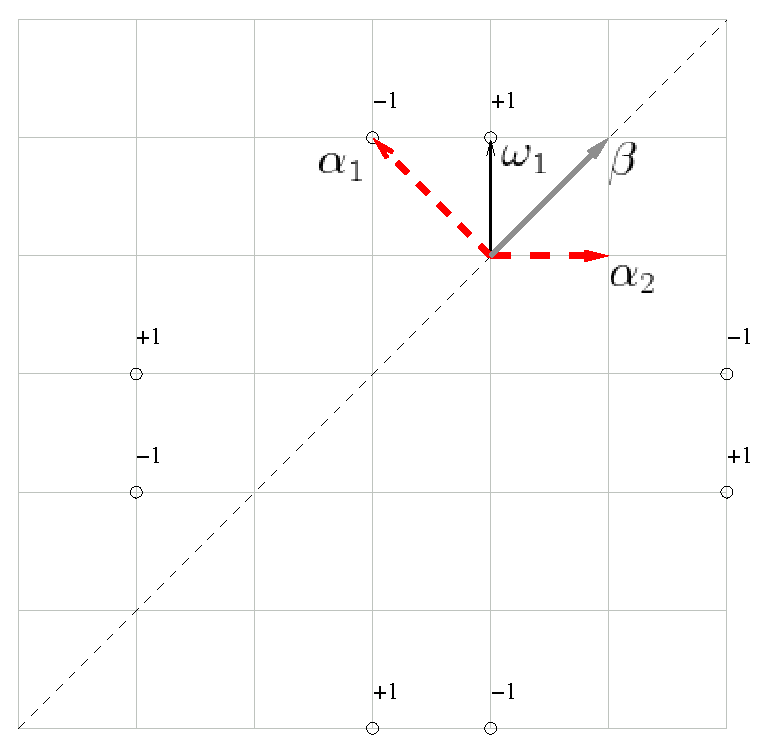
\includegraphics[width=80mm]{figure1.eps}
  }
  \caption{Regular embedding of $A_1$ into $B_2$}
  \label{fig:B2_A1}
\end{figure}
Circles indicate the weights of the singular element $\Psi^{(w_1)}$.
Now we are to factorise the Weyl group $W$ by $W_{\bot}=\left\{\omega_1\right\}$
and to construct the set $\left\{\omega(\mu+\rho)-\rho,\; \omega\in W_{\bot}\backslash W\right\}$.
\begin{figure}[t]
  \noindent\centering{
    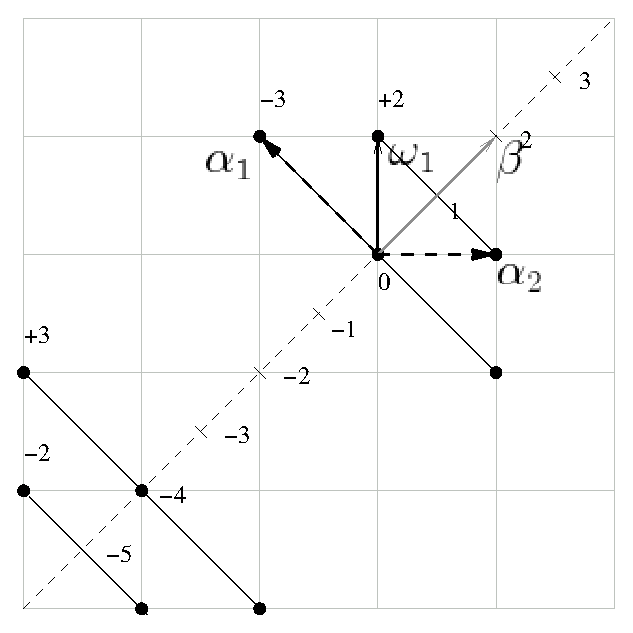
\includegraphics[width=80mm]{figure2.eps}
  }
  \caption{Anomalous weights and the corresponding $\mathfrak{a}_{\bot}=A_1$-modules for the embedding $A_1\subset B_2$}
  \label{fig:B2_A1_2}
\end{figure}
In the Figure \ref{fig:B2_A1_2} the weights of the corresponding
$\left(\mathfrak{a}_{\bot}=A_1\right)$-modules
$L^{\pi_{\mathfrak{a}_{\bot}}(\omega(\mu+\rho))-\rho_{\mathfrak{a}_{\bot}}}_{\mathfrak{a}_{\bot}}$
are indicated. Projecting them onto the root space of the subalgebra $\mathfrak{a}=A_1$
we get the anomalous weights and their multiplicities:
\begin{equation*}
  \label{eq:25}
  (1,2),\; (0,-3),\; (-4,3),\; (-5,-2).
\end{equation*}
For the set $\Gamma$ (using the definition \ref{fan-definition}) we have
\begin{equation*}
  \label{eq:22}
  \Gamma_{A_1\subset B_2}=\left\{ (1,2),\; (2,-1) \right\}.
\end{equation*}
Here the second component denotes the value of $s(\gamma)$.
Applying this fan inside the $\bar{C}^{(0)}_{\mathfrak{a}}$ we get zeros for the weights
greater than the first anomalous vector $(1)$, here $k^{(1,0)}_1=2$. For the last weight in $\bar{C}^{(0)}_{\mathfrak{a}}$ the formula (\ref{recurrent-relation}) gives
\begin{equation*}
  \label{eq:23}
  k^{(1,0)}_{0}=-1\cdot k^{(1,0)}_2 +2\cdot k^{(1,0)}_1 - 3\cdot \delta_{0,0} = 1.
\end{equation*}
The recurrence property defines the branching.

\subsection{Embedding of $B_2$ into $B_4$}
\label{sec:someth-high-dimens}
Consider the regular embedding $B_2 \longrightarrow B_4$.
The corresponding Dynkin diagrams are presented in the Figure \ref{fig:dynkin}.
\begin{figure}[h]
  \centering
  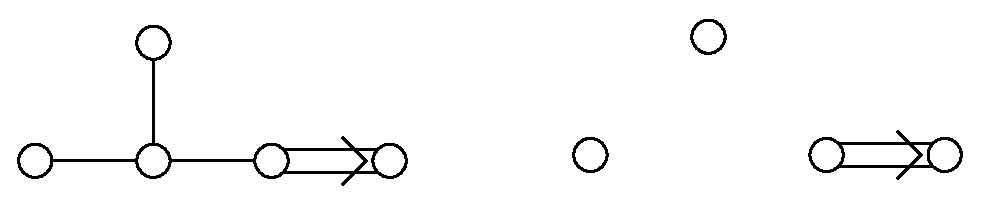
\includegraphics[width=50mm]{figure3.eps}
  \caption{The regular embedding $B_2\subset B_4$ described by dropping the node.}
  \label{fig:dynkin}
\end{figure}

In the orthogonal basis $\left\{e_1,\dots,e_4\right\}$ the simple roots and the positive roots of $B_4$ are
\begin{equation*}
  \label{eq:8}
 S_{B_4}= \{e_1 - e_2,\; e_2 - e_3,\; e_3 - e_4,\; e_4\}
\end{equation*}
\begin{eqnarray*}
  \label{eq:19}
 \Delta^+_{B_4}=\left\{ (e_1 - e_2,\; e_2 - e_3,\; e_3 - e_4,\; e_4,\; e_1 - e_3,\; e_2 - e_4,\; e_3 + e_4,\; e_3,\; e_1 - e_4,\;\right.\\
 \left. e_2 + e_4,\; e_2,\; e_1 + e_4,\; e_2 + e_3,\; e_1,\; e_1 + e_3,\; e_1 + e_2\right\}
\end{eqnarray*}
Correspondingly for the embedded subalgebra $\mathfrak{a}=B_2$ we have
\begin{equation*}
  \label{eq:26}
 S_{B_2}=\{e_3-e_4,e_4\}
\end{equation*}
and
\begin{equation*}
  \label{eq:27}
 \Delta^{+}_{\bot}= \left\{e_1-e_2,e_1+e_2,e_1,e_2\right\}
\end{equation*}
is the set of positive roots for the algebra $\mathfrak{a}_{\bot}=B_2$.
\begin{figure}[t]
  \centering
    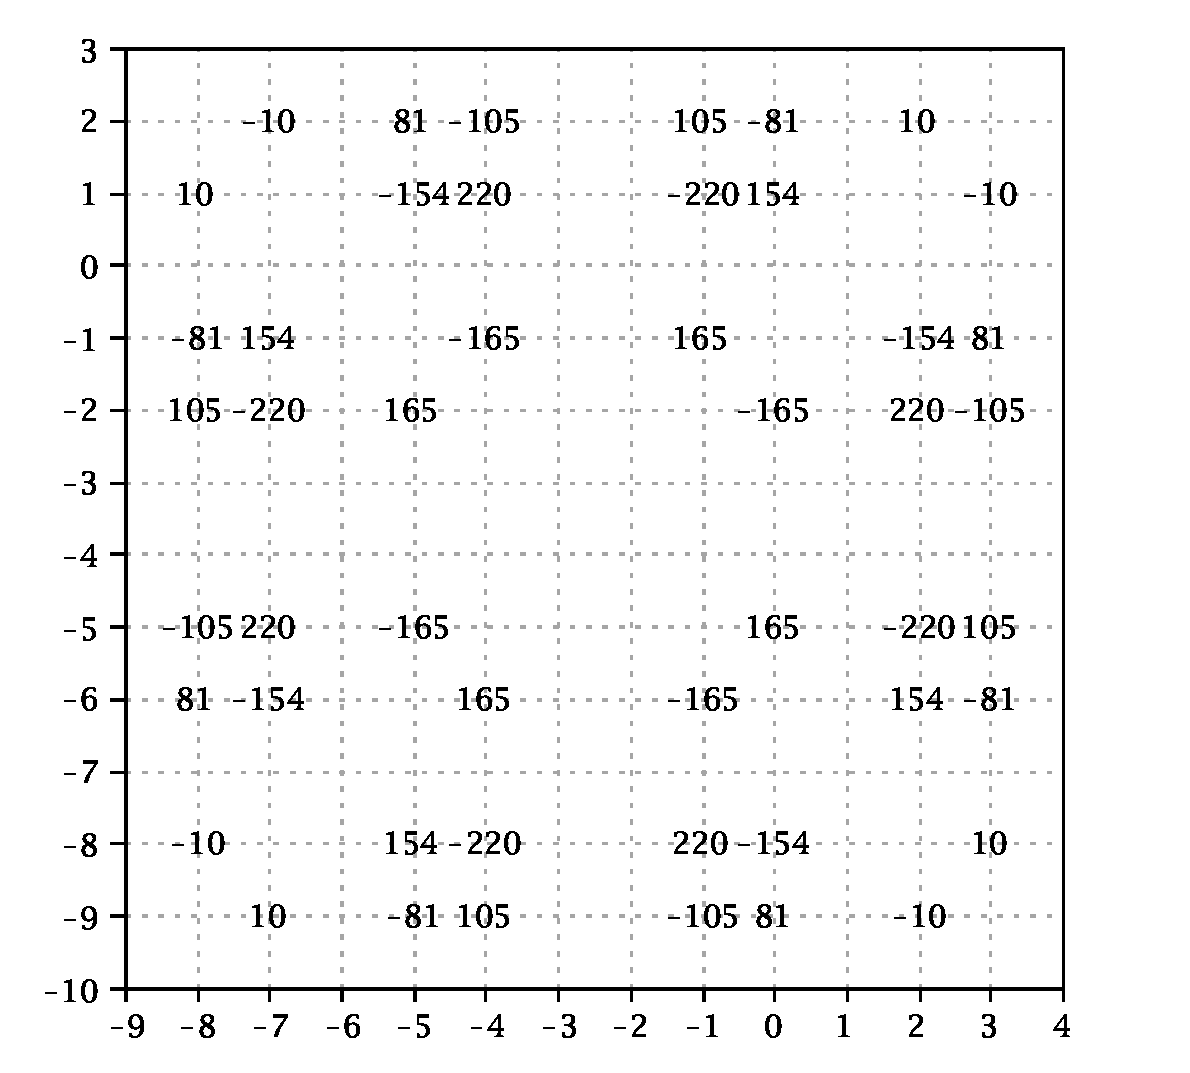
\includegraphics[width=100mm,height=90mm]{figure4.eps}
  \caption{Projected weights $-\frac{1}{s(\gamma_0)}\pi_{B_2}\left(\hat \Psi^{(0,1,0,2)}_{B_4}\right)$
  with the dimensions of the corresponding $\mathfrak{a}_{\bot}$-modules.}
  \label{fig:B4B2anom}
\end{figure}

\begin{figure}[b]
  \centering
  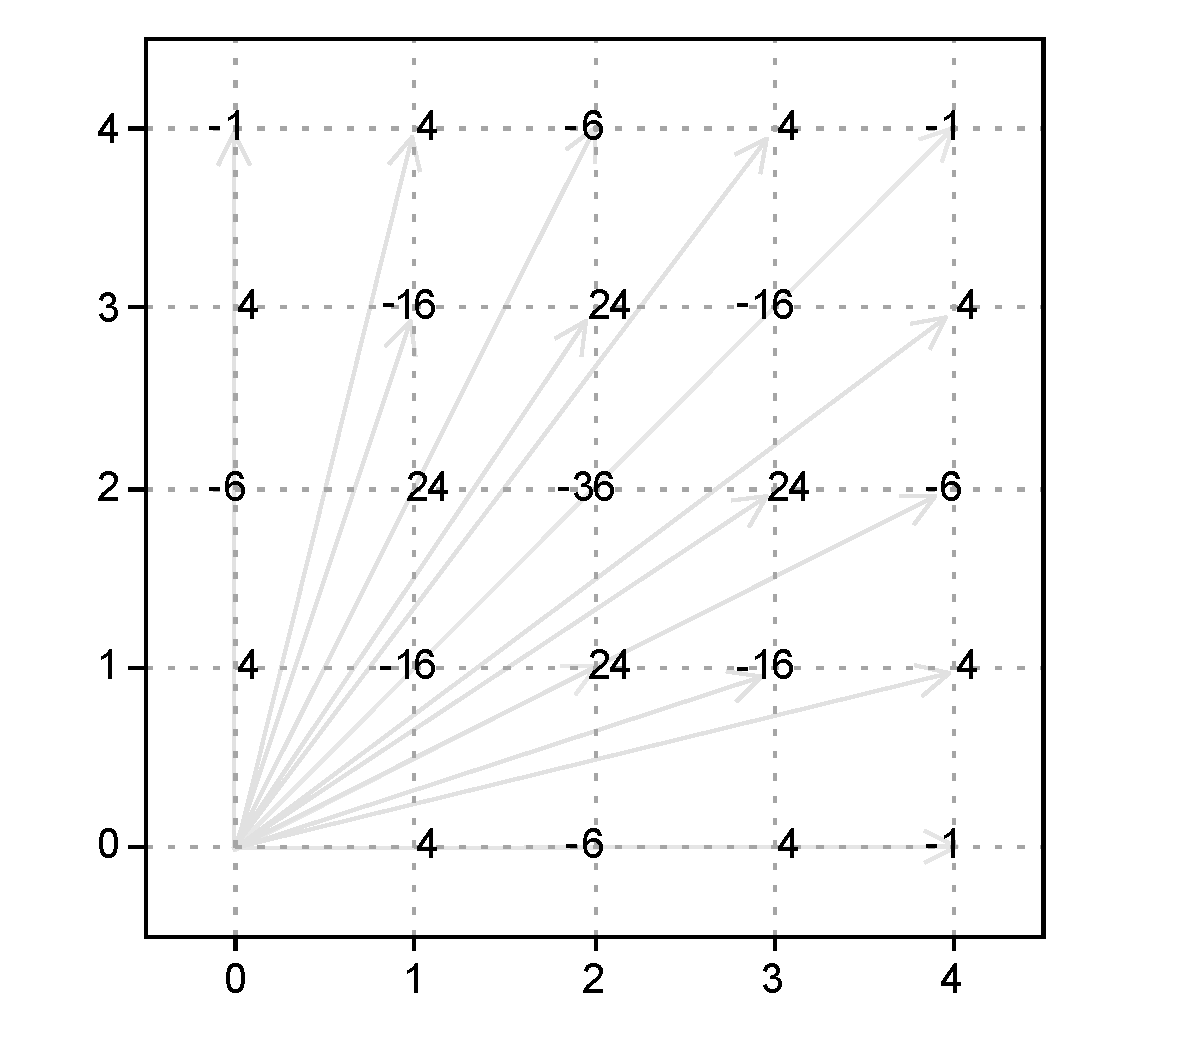
\includegraphics[height=80mm]{figure5.eps}
  \caption{The fan for $B_2\subset B_4$}
  \label{fig:B4B2Fan}
\end{figure}
Using the definition (\ref{fan-defined}) we obtain the fan
$\Gamma_{B_2\subset B_4}$ with the corresponding values $s(\gamma+\gamma_0)$,
depicted in the Figure \ref{fig:B4B2Fan}.


Consider the $B_4$-module $L^{\mu}$ with the highest weight $\mu=(0,1,0,2)=2
e_1 + 2 e_2 + e_3 + e_4$; $\mathrm{dim}(L^{(0,1,0,2)})=2772$.
To find the branching coefficients we need to compute the anomalous weights of
$L^{\mu}_{B_4}$, select the weights belonging to $\bar{C}^{\left( 0 \right)}_{\mathfrak{a}_{\bot}}$
and compute the dimensions of the corresponding $\mathfrak{a}_{\bot}$-modules.
The set of the anomalous weights $\left\{ \omega(\mu+\rho)-\rho,\; \omega\in W\right\}$
contains 384 vectors.

We are to select the weights $\psi \in \omega(\mu+\rho)$  with the property
$\pi_{\mathfrak{a}_{\bot}} \left(  \psi \right) \in \bar{C}^{\left( 0 \right)}_{\mathfrak{a}_{\bot}}$.
It means that the scalar product of these weights with all the roots in $\Delta^{+}_{\bot}$ is nonnegative.

To compute the dimensions of the corresponding
$\mathfrak{a}_{\bot}$-modules we need to project each selected weight
onto the root space $\Delta^{+}_{\bot}$, subtract
$\rho_{\mathfrak{a}_{\bot}}$ and apply the Weyl dimension formula. The result is shown in the Figure \ref{fig:B4B2anom}.

Applying the recurrent relation (\ref{recurrent-relation}) we obtain the
following branching coefficients:
\begin{eqnarray*}
  \label{eq:24}
  \pi_{\mathfrak{a}} \left(ch L^{(0,1,0,2)}_{B_4}\right) = 6 \; ch L^{(0,0)}_{B_2}+ 60
  \; ch L_{B_2}^{(0,2)}+ 30 \; ch L_{B_2}^{(1,0)}+ 19 \; ch L_{B_2}^{(2,0)}+\\
  40 \; ch L_{B_2}^{(1,2)}+ 10 \; ch L_{B_2}^{(2,2)}.
\end{eqnarray*}
%\newpage
\section{Applications to the conformal field theory}
\label{sec:phys-appl}

\subsection{Conformal embeddings}
\label{sec:conformal-embeddings}

Branching coefficients for an embedding of affine Lie algebra into
affine Lie algebra can be used to construct modular invariant
partition functions for Wess-Zumino-Novikov-Witten models in conformal field theory
(\cite{difrancesco1997cft}, \cite{Walton:1999xc}, \cite{walton1989conformal}, \cite{schellekens1986conformal}).
In these models current algebras are affine Lie algebras.

The modular invariant partition function is crucial for the conformal theory to be valid
on the torus and higher genus Riemann surfaces. It is important for the applications of
CFT to the string theory and to the critical phenomena description.

The simplest modular-invariant partition function has the diagonal form:
\begin{equation*}
  \label{eq:34}
   Z(\tau)=\sum_{ \mu\in P^{+}_{\mathfrak{g}}} \chi_{\mu}(\tau)\bar \chi_{\mu}(\bar \tau)
\end{equation*}
Here the sum is over the set of the highest weights of integrable modules in a WZW-model
and $\chi_{\mu}(\tau)$ are the normalized characters of these modules.

To construct the nondiagonal modular invariants is not an easy problem,
although for some models the complete classification of modular invariants is known \cite{1994hepthGannon,1995JMPGannon}.

Consider the Wess-Zumino-Witten model with the affine Lie algebra $\mathfrak{a}$.
Nondiagonal modular invariants for this model can be constructed from the diagonal
invariant if there exists an affine algebra $\mathfrak{g}$ such that $\mathfrak{a}\subset\mathfrak{g}$.
Then we can replace the characters of the $\mathfrak{g}$-modules in the diagonal
modular invariant partition function (\ref{eq:36})
by the decompositions
\begin{equation*}
  \label{eq:32}
\sum_{\nu \in P^{+}_{\mathfrak{a}}}b^{(\mu)}_{\nu} \chi_{\nu}
\end{equation*}
containing the modified characters $\chi_{\nu}$ of the corresponding $\mathfrak{a}$-modules.
Thus we obtain the nondiagonal modular-invariant  partition function for the theory with
the current algebra $\mathfrak{a}$,
\begin{equation}
  \label{eq:36}
   Z_{\mathfrak{a}}(\tau)=\sum_{ \nu,\lambda\in P^{+}_{\mathfrak{a}}} \chi_{\nu}(\tau)M_{\nu\lambda}\bar \chi_{\lambda}(\bar \tau).
\end{equation}

The effective reduction procedure is crucial for this construction.
The embedding is required to preserve the conformal invariance.
Let $X^{\alpha_j}_{-n_j}$ and $\tilde{X}^{\alpha'_j}_{-n_j}$ be the lowering generators for
$\mathfrak{g}$ and for $\mathfrak{a}\subset\mathfrak{g}$ correspondingly.
Let $\pi_{\mathfrak{a}}$ be the projection operator of
$\pi_{\mathfrak{a}}:\mathfrak{g}\longrightarrow \mathfrak{a}$.
In the theory attributed to $\mathfrak{g}$ with the vacuum $\left|\lambda\right>$
the states can be described as
\begin{equation*}
  \label{eq:109}
  X^{\alpha_1}_{-n_1}X^{\alpha_2}_{-n_2}\dots\left|\lambda\right>\quad n_1\geq n_2\geq \dots>0.
\end{equation*}
And for the sub-algebra $\mathfrak{a}$ the corresponding states are
\begin{equation*}
  \label{eq:110}
  \tilde{X}^{\alpha'_1}_{-n_1}\tilde{X}^{\alpha'_2}_{-n_2}\dots\left|\pi_{\mathfrak{a}}(\lambda)\right>.
\end{equation*}
The $\mathfrak{g}$-invariance of the vacuum entails its $\mathfrak{a}$-invariance,
but this is not the case for the energy-momentum tensor. So the energy-momentum tensor of the larger theory
should contain only the generators $\tilde{X}$. Then the relation
\begin{equation}
  \label{eq:2}
  T_{\mathfrak{g}}(z)=T_{\mathfrak{a}}(z)
\end{equation}
leads to the equality of the central charges
\begin{equation*}
  \label{eq:33}
  c(\mathfrak{g})=c(\mathfrak{a})
\end{equation*}
and to the equation
\begin{equation}
  \label{eq:111}
  \frac{k\;\mathrm{dim}\,\mathfrak{g}}{k+g}=\frac{x_e k\; \mathrm{dim}\,\mathfrak{a}}{x_ek+a}.
\end{equation}
Here $x_e$ is the embedding index and $g$, $a$ are the dual Coxeter numbers for the  corresponding algebras.

It can be demonstrated that the solutions of the equation (\ref{eq:111}) exist only
for the level $k=1$ \cite{difrancesco1997cft}.

The complete classification of conformal embeddings is given in \cite{schellekens1986conformal}.

The relation (\ref{eq:111}) and the asymptotics of the branching functions can be used
to prove the finite reducibility theorem \cite{kac1988modular}.
It states that for the conformal embedding  $\mathfrak{a}\subset\mathfrak{g}$
only finite number of branching coefficients have nonzero values.

\begin{mynote} The orthogonal subalgebra $\mathfrak{a}_{\bot}$ is always empty for the conformal embeddings $\mathfrak{a}\subset \mathfrak{g}$.
\begin{proof}
Consider the modes expansion of the energy-momentum tensor
\begin{equation*}
\label{eq:47}
  T(z)=\frac{1}{2(k+h^v)}\sum_n z^{-n-1}L_n.
\end{equation*}
The modes $L_n$ are constructed as combination of normally-ordered products of the generators of $\mathfrak{g}$,
\begin{equation*}
\label{eq:48}
  L_n=\frac{1}{2(k+h^v)}\sum_{\alpha}\sum_m:X^{\alpha}_m X^{\alpha}_{n-m}: \; .
\end{equation*}
In the case of a conformal embedding energy-momentum tensors are to be equal (\ref{eq:2}).

The substitution of the generators of $\mathfrak{a}$  in terms of the generators of $\mathfrak{g}$ into these combinations  should give the energy-momentum tensor $T_{\mathfrak{g}}$. But if the set of the generators $\Delta_{\bot}$ is not empty this is not possible, since $T_{\mathfrak{g}}$ contains the combinations of the generators $X^{\alpha}_n, \; \alpha\in \Delta_{\bot}$.
\end{proof}
\end{mynote}
\subsubsection{Special embedding $\hat{A}_1\subset\hat{A}_2$}
\label{sec:spec-embedd-hata_1s}
Consider the case where both $\mathfrak{g}$ and $\mathfrak{a}$ are affine Lie algebras:
$\hat{A}_1 \longrightarrow \hat{A}_2$ and the injection is the affine extension of the
special injection $A_1 \longrightarrow A_2$ with the embedding index $x_e=4$.
As far as the $\mathfrak{g}$-modules to be considered are of level one,
the $\mathfrak{g}$-modules will be of level $\tilde{k}=kx_e=4$.

There exist three level one fundamental weights in the weight space of $\hat{A}_2$.
It is easy to see that the set $\Delta_{\bot}$ is empty and the subalgebra $\mathfrak{a}_{\bot}=0$.

Using the definition (\ref{fan-defined})  we construct the fan $\Gamma_{\hat A_1\to\hat A_2}$
and the function $s(\gamma+\gamma_0)$ (see the Figure \ref{fig:AffineA2A1Fan}).

\begin{figure}[h!bt]
  \centering
  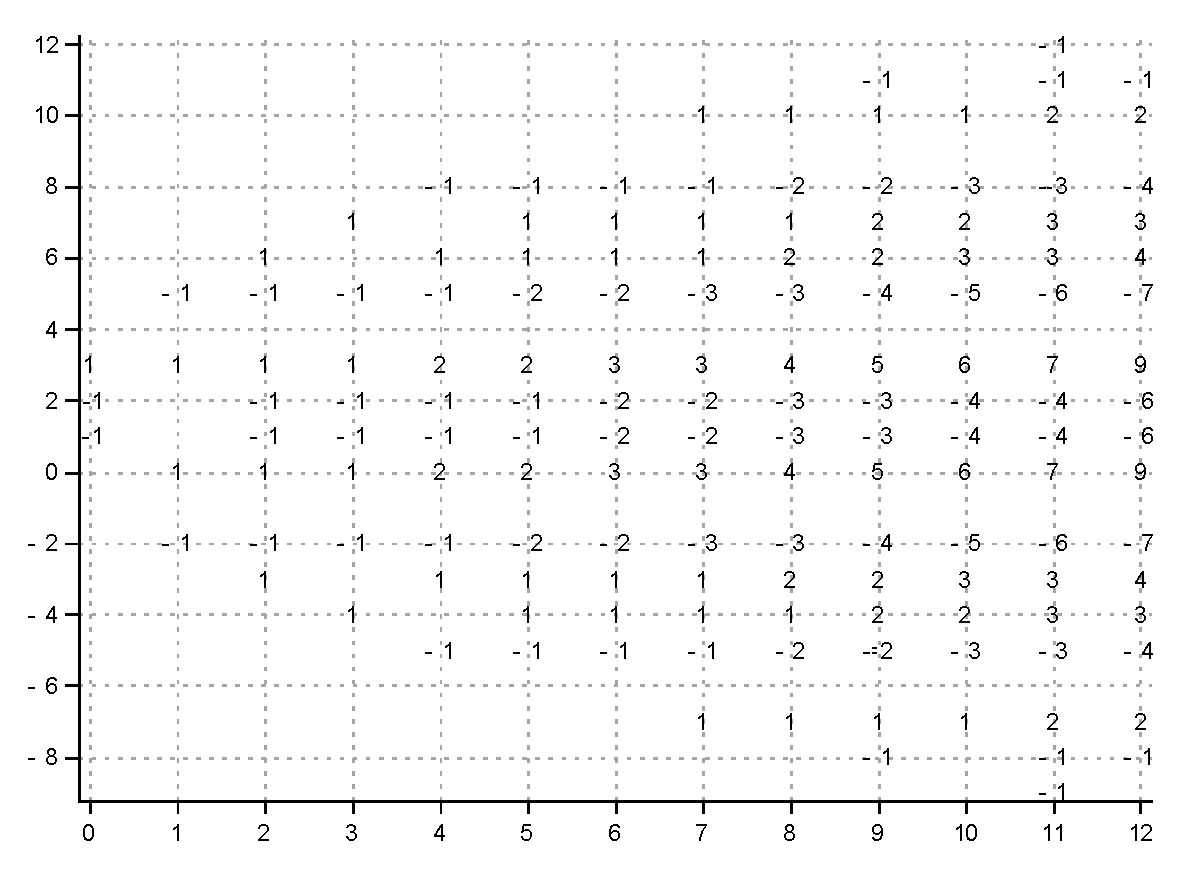
\includegraphics[width=135mm]{figure6.eps}
  \caption{The fan and $s(\gamma+\gamma_0)$ for $\hat{A_1}\longrightarrow \hat{A_2}$}
  \label{fig:AffineA2A1Fan}
\end{figure}

Let us consider the module $L^{w_0=(0,0;1;0)}$. Here we use the (finite part; level; grade)
presentation of the highest weight and the finite part
coordinates are the Dynkin indices (see section(\ref{sec:notation})).

The set $\widehat{\Psi^{(w_0)}}$  is depicted in the Figure
\ref{fig:affine_A2_anom_point} up to the sixth grade.
The weights $\omega (w_0+\rho)-\rho$ are marked by crosses when $\epsilon(\omega)=1$ and
by diamond when $\epsilon(\omega)=-1$. Simple roots of the classical subalgebra $A_2$ are
grey and the grey diagonal plane corresponds to the Cartan subalgebra of
the embedded algebra $\hat{A}_1$.

\begin{figure}[h!tb]
%  \hspace*{-2cm}
  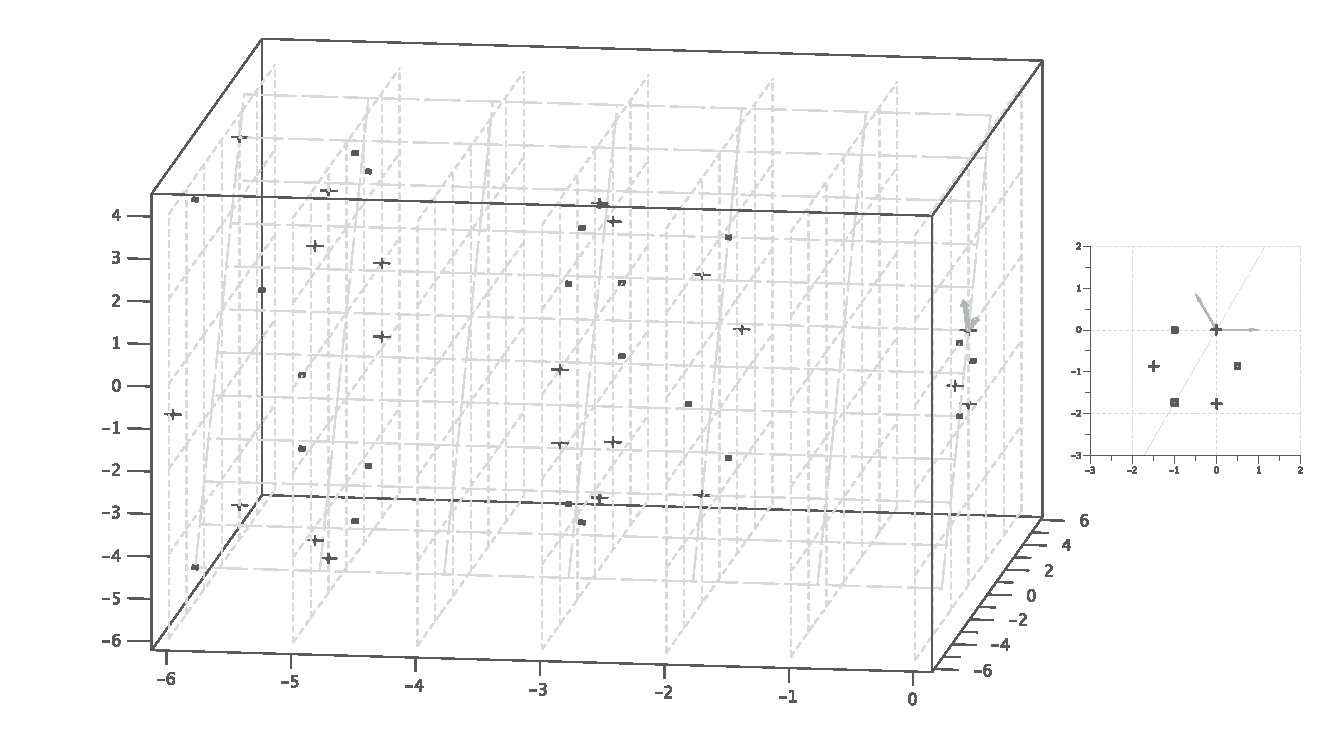
\includegraphics[width=140mm]{figure7.eps}
  \caption{The anomalous weights of the module $L^{(0,0;1;0)}_{\hat{A_2}}$}
  \label{fig:affine_A2_anom_point}
\end{figure}

The next step is to project the anomalous weights to $P_{\hat A_1}$.
The result is presented in the Figure \ref{fig:AffineA2_A1_anom_proj} up to the twelfth grade.
\begin{figure}[h!tb]
  \centering
  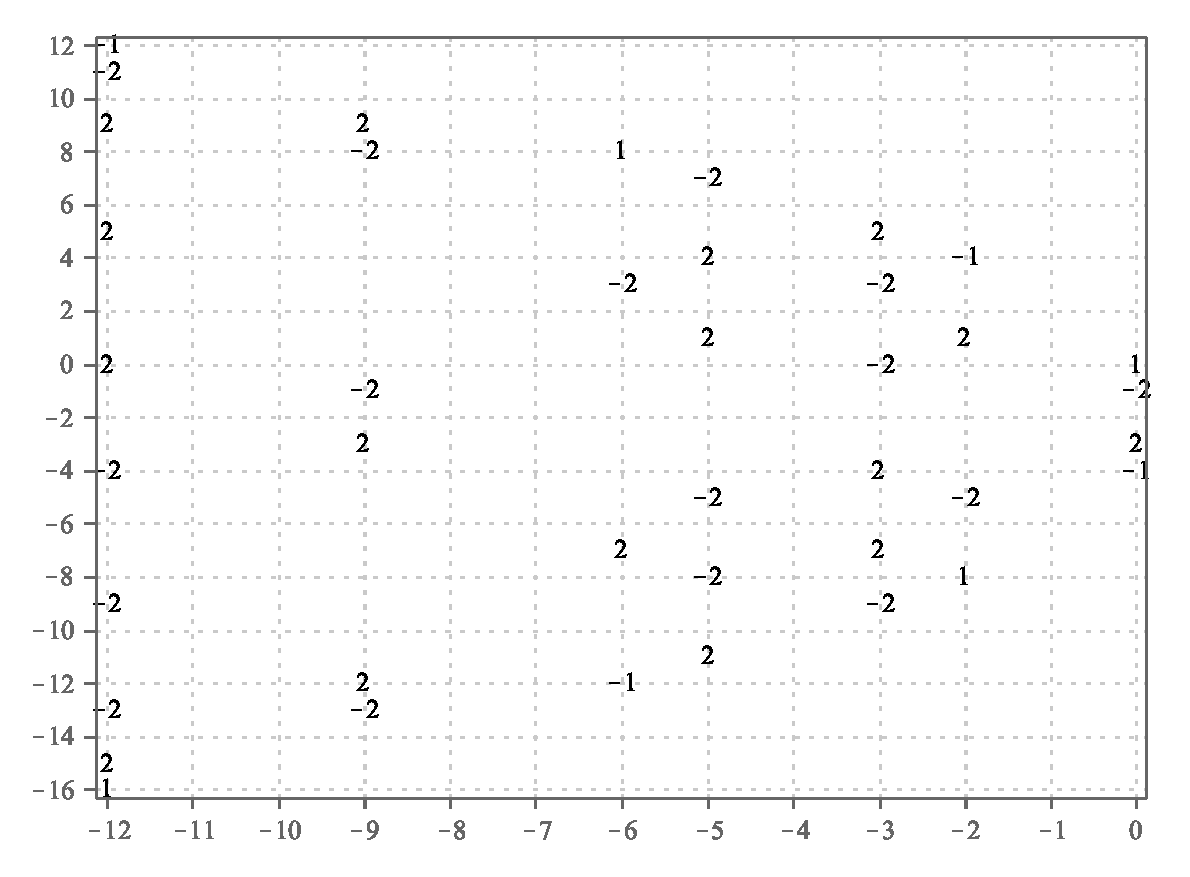
\includegraphics[width=130mm]{figure8.eps}
  \caption{Projected anomalous weights of $L^{(0,0;1;0)}_{\hat{A_2}}$.}
  \label{fig:AffineA2_A1_anom_proj}
\end{figure}


Using the recurrent relation for the anomalous branching coefficients
we get the result presented in Figure \ref{fig:AffineA2_A1_branching}.
\begin{figure}[h!tb]
  \centering
  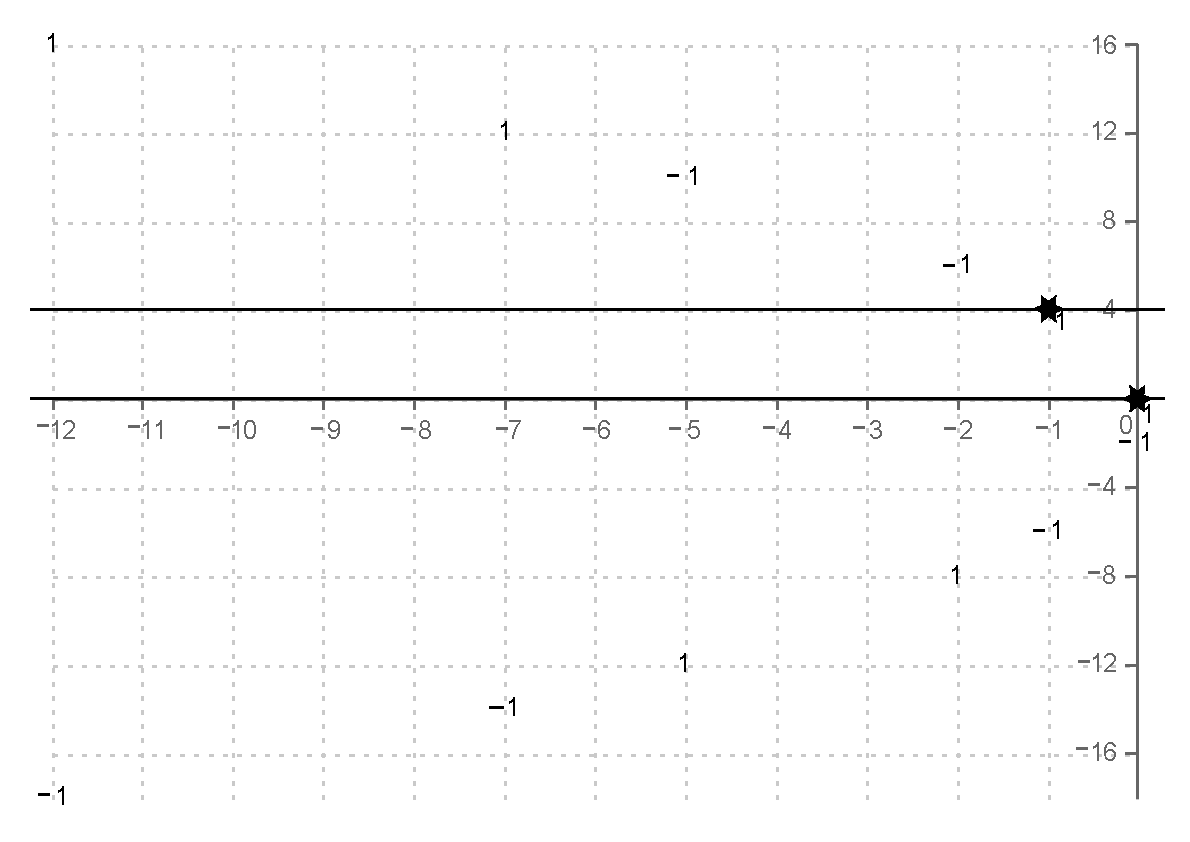
\includegraphics[width=130mm]{figure9.eps}
  \caption{Anomalous branching coefficients for $\hat{A_1}\subset \hat{A_2}$}
  \label{fig:AffineA2_A1_branching}
\end{figure}
Inside the Weyl chamber $\bar{C}_{\hat{A}_1}$
(its boundaries are indicated in the Figure \ref{fig:AffineA2_A1_branching})
there are only two nonzero anomalous weights and both have multiplicity 1.
These are the highest weights of $\mathfrak{a}$-submodules and their branching
coefficients. So the finite reducibility theorem holds and we get the decomposition
\begin{equation*}
  \label{eq:43}
  L^{(0,0;1;0)}_{\hat{A_2}\downarrow \hat{A_1}}= L_{\hat{A_1}}^{(0;4;0)}\oplus L_{\hat{A_1}}^{(4;4;0)}.
\end{equation*}

For the other irreducible modules of level one  we get the trivial
branching
\begin{equation*}
  \label{eq:44}
   L^{(1,0;1;0)}_{\hat{A_2}\downarrow \hat{A_1}}= L_{\hat{A_1}}^{(2;4;0)},\\
   L^{(0,1;1;0)}_{\hat{A_2}\downarrow \hat{A_1}}= L_{\hat{A_1}}^{(2;4;0)}.
\end{equation*}

Using these results the modular-invariant partition function is easily found,
\begin{equation*}
  \label{eq:45}
  Z=\left|\chi_{(4;4;0)}+\chi_{(0;4;0)}\right|^2+2\chi_{(2;4;0)}^2.
\end{equation*}

\subsection{Coset models}
\label{sec:coset-models}

Coset models \cite{Goddard198588} tightly connected with the gauged WZW-models are actively studied
in string theory, especially in string models on anti-de-Sitter space
\cite{Maldacena:2000hw,Maldacena:2000kv,Maldacena:2001km,Maldacena:2001ky,Aharony:1999ti}.
The characters in coset models are proportional to the branching functions,
\begin{equation}
  \label{eq:31}
  \chi^{(\mu)}_{\nu}(\tau)=e^{2\pi i \tau (m_{\mu}-m_{\nu})} b^{(\mu)}_{\nu}(\tau),
\end{equation}
with
\begin{equation*}
  \label{eq:46}
  m_{\mu}=\frac{\left|\mu+\rho\right|^2}{2(k+g)}-\frac{\left|\rho\right|^2}{2g}.
\end{equation*}
The problem of the branching functions construction in the coset models was considered
in  \cite{Dunbar:1992gh}, \cite{Hwang:1994yr}, \cite{lu1994branching}.

Let us return to the example \ref{sec:regul-embedd-a_1} and consider the affine extension of the injection
$A_1 \longrightarrow B_2$.
Since this embedding is regular and $x_e=1$, the subalgebra modules and the initial module are of the same level.
The set $\Delta^{+}_{\bot}$ of the orthogonal positive roots with the zero projection
on the root space of the subalgebra $\hat{A_1}$ is the same as in the finite-dimensional case.

Using the definition (\ref{fan-defined}) we get the fan
$\Gamma_{\hat{A_1} \longrightarrow  \hat{B_2} }$
with the corresponding values $s(\gamma+\gamma_0)$ (see the Figure \ref{fig:AffineB2A1Fan}).
We restricted the computation to the twelfth grade.
\begin{figure}[h!bt]
  \centering
  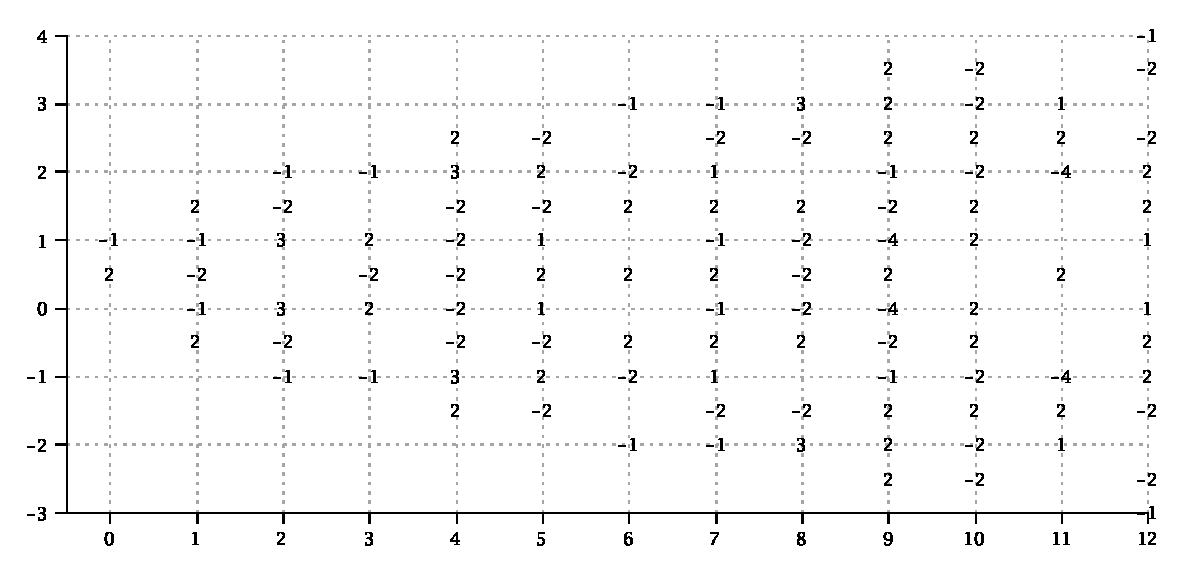
\includegraphics[width=135mm]{figure10.eps}
  \caption{The fan for $\hat{A_1}\subset \hat{B_2}$}
  \label{fig:AffineB2A1Fan}
\end{figure}


Consider the level one module $L^{\left( 1,0;1;0 \right)}_{\hat{B_2}}$  with the highest weight $w_1=(1,0;1;0)$,
where the finite part coordinates are in the orthogonal basis $e_1,e_2$.
The set of anomalous weights for this module up to the sixth grade is presented in the Figure \ref{fig:affine_B2_anom_point}.
In the grade zero it is exactly the set of the anomalous weights for the embedding of
the classical Lie algebras $A_1\subset B_2$ that can be seen in the  Figure \ref{fig:B2_A1}.
The weights $\omega (w_1+\rho)-\rho$ are marked by crosses if $\epsilon(\omega)=1$ and by circles otherwise.
Simple roots of the classical subalgebra $B_2$ are grey and grey diagonal plane corresponds to the Cartan subalgebra
of the embedded algebra $\hat{A}_1$.

\begin{figure}[h!tb]
%  \hspace*{-2cm}
  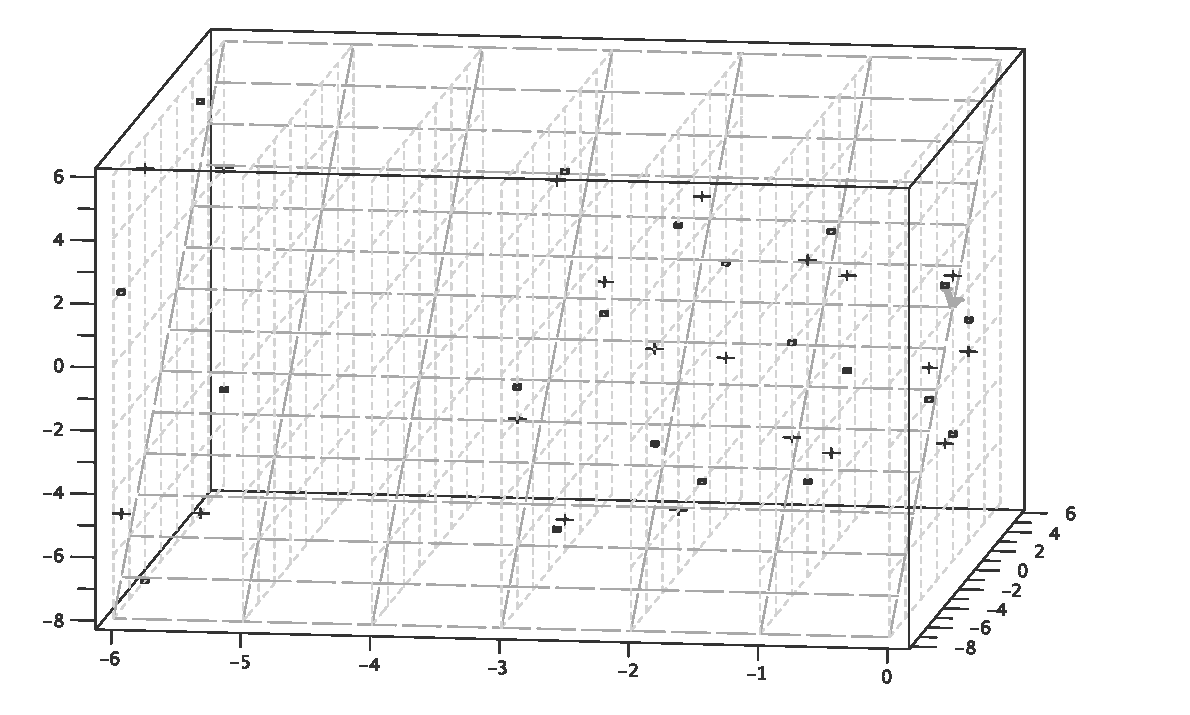
\includegraphics[width=140mm]{figure11.eps}
  \caption{The anomalous weights of $L^{(1,0;1;0)}_{\hat B_2 }$.
  The weights in the zero grade can be seen in the Figure \ref{fig:B2_A1}}.
  \label{fig:affine_B2_anom_point}
\end{figure}

According to the algorithm \ref{sec:algorithm} we project the anomalous weights to
$P_{\hat{A_1}}$ and find the dimensions of the corresponding
$\mathfrak{a}_{\bot}$-modules $L^{\pi_{\mathfrak{a}_{\bot}}(\omega(\mu+\rho))-\rho_{\mathfrak{a}_{\bot}}}_{\mathfrak{a}_{\bot}}$.
The result is presented in the Figure
\ref{fig:AffineB2_A1_anom_proj} up to the twelfth grade.
\begin{figure}[h!tb]
  \centering
  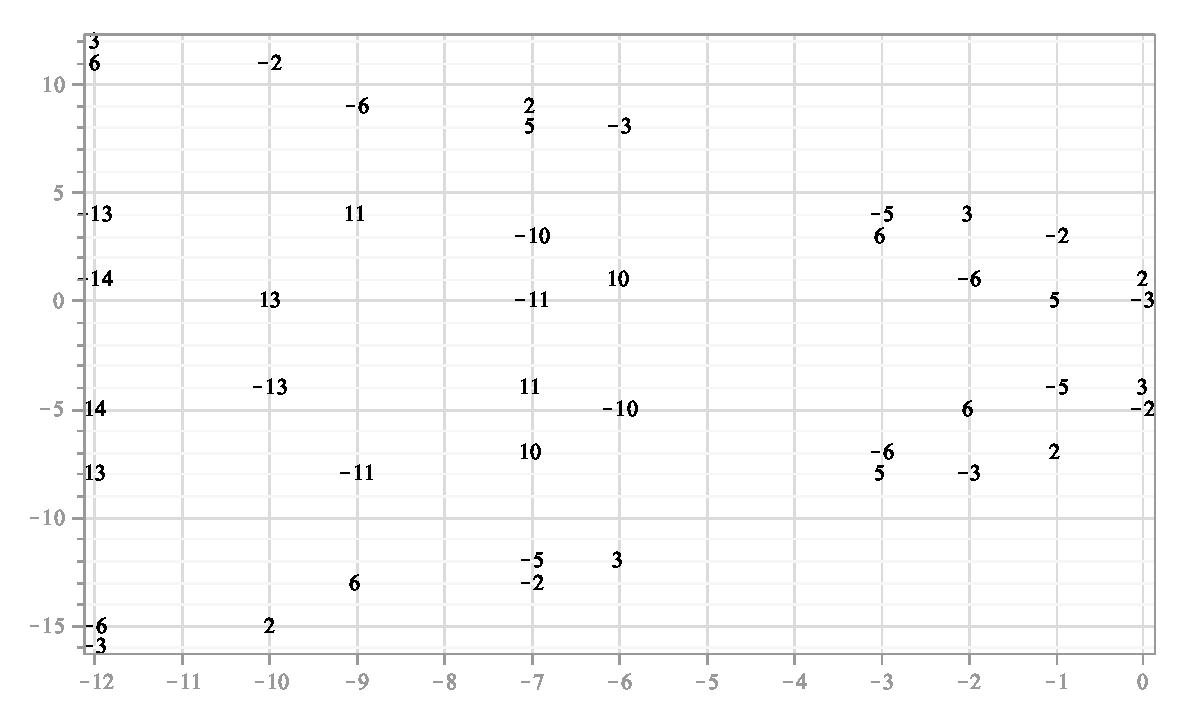
\includegraphics[width=120mm]{figure12.eps}
  \caption{The projected anomalous weights $\pi_{\hat A_1}\left(\Psi^{(1,0;1;0)}_{\hat B_2}\right)$ and the dimensions of $\mathfrak{a}_{\bot}$-modules.}
  \label{fig:AffineB2_A1_anom_proj}
\end{figure}

Notice that here the lowest weight  $\gamma_0$ of the fan  is zero, since we have excluded all the roots of $\Delta^{+}_{\bot}$ from the defining relation (\ref{fan-defined}).

\begin{figure}[h!bt]
  \centering
  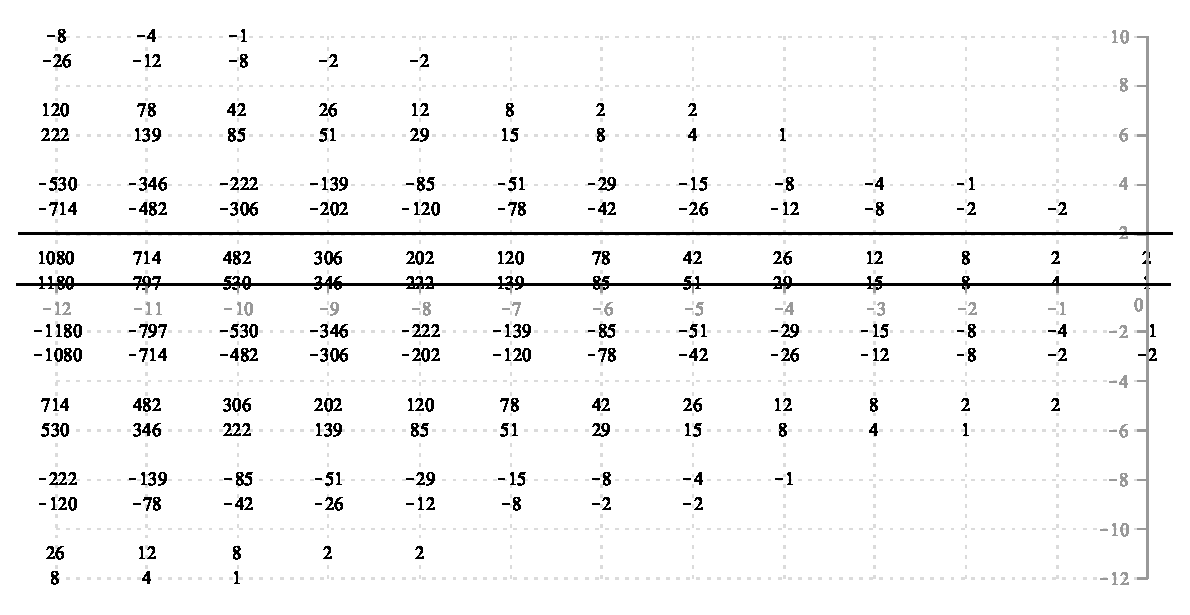
\includegraphics[width=120mm]{figure13.eps}
  \caption{Anomalous branching coefficients for $\hat{A_1}\subset \hat{B_2}$}
  \label{fig:AffineB2_A1_branching}
\end{figure}

The multiplicities of the weights inside the  Weyl chamber
$\bar{C}^{\left( 0 \right)}_{\hat{A_1}}$
are the branching coefficients (up to the twelfth grade),
\begin{eqnarray*}
  \label{eq:28}
  L^{w_1}_{\hat{B_2}\downarrow \hat{A_1}}=2 L_{\hat{A_1}}^{w_1}\oplus 1 L_{\hat{A_1}}^{w_0}\oplus 4 L_{\hat{A_1}}^{w_0-\delta}\oplus\\
    2 L_{\hat{A_1}}^{w_1-\delta}\oplus 8 L_{\hat{A_1}}^{w_0-2\delta}\oplus
    8 L_{\hat{A_1}}^{w_1-2\delta}\oplus 15 L_{\hat{A_1}}^{w_0-3\delta}\oplus\\
    12 L_{\hat{A_1}}^{w_1-3\delta}\oplus 26 L_{\hat{A_1}}^{w_1-4\delta}\oplus
    29 L_{\hat{A_1}}^{w_0-4\delta}\oplus 51 L_{\hat{A_1}}^{w_0-5\delta}\oplus\\
    42 L_{\hat{A_1}}^{w_1-5\delta}\oplus 78 L_{\hat{A_1}}^{w_1-6\delta}\oplus
    85 L_{\hat{A_1}}^{w_0-6\delta}\oplus 120 L_{\hat{A_1}}^{w_1-7\delta}\oplus\\
    139 L_{\hat{A_1}}^{w_0-7\delta}\oplus 202 L_{\hat{A_1}}^{w_1-8\delta}\oplus
    222 L_{\hat{A_1}}^{w_0-8\delta}\oplus 306 L_{\hat{A_1}}^{w_1-9\delta}\oplus\\
    346 L_{\hat{A_1}}^{w_0-9\delta}\oplus 530 L_{\hat{A_1}}^{w_0-10\delta}\oplus
    482 L_{\hat{A_1}}^{w_1-10\delta}\oplus 714 L_{\hat{A_1}}^{w_1-11\delta}\oplus\\
    797 L_{\hat{A_1}}^{w_0-11\delta}\oplus 1080 L_{\hat{A_1}}^{w_1-12\delta}\oplus
    1180 L_{\hat{A_1}}^{w_0-12\delta}\oplus \dots
\end{eqnarray*}
This result can be presented as the set of branching functions:
\begin{eqnarray*}
  \label{eq:29}
  \begin{array}{cc}
    b^{(w_1)}_{0}= & 1 + 4\,q^{1}+ 8\,q^{2}+ 15\,q^{3}+ 29\,q^{4}+ 51\,q^{5}+ 85\,q^{6}+ 139\,q^{7}+\\
     &222\,q^{8}+ 346\,q^{9}+ 530\,q^{10}+ 797\,q^{11}+ 1180\,q^{12}+\dots\\
  \end{array}\\
  \begin{array}{cc}
    b^{(w_1)}_{1}= &2+2\,q^{1}+8\,q^{2}+12\,q^{3}+26\,q^{4}+42\,q^{5}+78\,q^{6}+120\,q^{7}+\\
    & 202\,q^{8}+306\,q^{9}+482\,q^{10}+714\,q^{11}+1080\,q^{12}+\dots
  \end{array}
\end{eqnarray*}
Here $q=\exp (2\pi i \tau)$ and the lower index enumerates the branching functions according
to their highest weights in $P^+_{\hat{A_1}}$.
These are the fundamental weights $w_0=\lambda_0=(0,1,0),\; w_1=\alpha/2=(1,1,0)$.

Now we can use the relation (\ref{eq:31}) to get the expansion of the $B_2/A_1$-coset characters:
\begin{equation*}
  \label{eq:35}
  \begin{array}{cc}
    \chi^{(w_1)}_{1}(q)= & q^{\frac{7}{12}}\left( 2+2\,q^{1}+8\,q^{2}+12\,q^{3}+26\,q^{4}+42\,q^{5}+78\,q^{6}+120\,q^{7}+\right. \\
    & \left. 202\,q^{8}+306\,q^{9}+482\,q^{10}+714\,q^{11}+1080\,q^{12}+\dots \right)\\
    \chi^{(w_1)}_{0}(q) = & q^{\frac{5}{6}}\left(1 + 4\,q^{1}+ 8\,q^{2}+ 15\,q^{3}+ 29\,q^{4}+ 51\,q^{5}+ 85\,q^{6}+ 139\,q^{7}+\right. \\
    &\left. 222\,q^{8}+ 346\,q^{9}+ 530\,q^{10}+ 797\,q^{11}+ 1180\,q^{12}+\dots\right)
  \end{array}
\end{equation*}

Further amelioration of the algorithm can be achieved by using
the folded fan technique \cite{il2010folded} to get the explicit expression
for the branching functions and the corresponding coset characters in conformal field theory.

\section{Conclusion}
\label{sec:conclusion}
We have demonstrated that the injection fan technique can be used to deal with the nonmaximal subalgebras.
It was found out that for such subalgebras an auxiliary subset $\Delta^{+}_{\bot}$ must be extracted
from the set of positive roots $\Delta_{\mathfrak{g}}^{+}$.
The role of the subset $\Delta^{+}_{\bot}$ is to modify both the injection fan (formed here by the
weights $\left(\Delta_{\mathfrak{g}}^{+} \setminus  \Delta_{\mathfrak{a}}^{+}\right) \setminus \Delta^{+}_{\bot}$)
and the anomalous weights of the initial module.
This modification reduces to a simple procedure:
the anomalous weights multiplicities are to be substituted by the dimensions of the corresponding ${\mathfrak{a}}_{\bot}$-modules.

The efficiency of the injection fan algorithm was verified.
Its possible applications to some physical problems were discussed.
In particular we considered the construction of modular-invariant partition functions
in the framework of conformal embedding method and the coset construction in the rational conformal field theory.
This construction is useful in the study of WZW-models
emerging in the context of the AdS/CFT correspondence \cite{Maldacena:2000hw,Maldacena:2000kv,Maldacena:2001km}.

\section{Acknowledgements}
The work was supported in
part by RFFI grant N 09-01-00504 and the National Project RNP.2.1.1./1575.

\section*{References}
\bibliography{article}{}
\bibliographystyle{iopart-num}

\end{document}
